\newcommand{\nauticleversion}{1.0.170221}
\newcommand{\installer}{install-\nauticleversion{}.sh}
\newcommand{\uninstaller}{uninstall-\nauticleversion{}.sh}
\newcommand{\execname}{\textbf{nauticle}}

\documentclass[a4paper,12pt,openany]{book}
% \documentclass[a4paper,12pt,openany]{paper}
\usepackage{courier}
\usepackage{gensymb}
\usepackage[utf8]{inputenc}
\usepackage[T1]{fontenc}
\usepackage[english]{babel} % If you write in English
\usepackage{a4wide}
\usepackage{graphicx}
\graphicspath{{images/}}
\usepackage{subfig}
\usepackage{tikz}
\usetikzlibrary{shapes,arrows}
\usepackage{pgfplots}
\pgfplotsset{compat=newest}
\pgfplotsset{plot coordinates/math parser=false}
\newlength\figureheight
\newlength\figurewidth
\pgfkeys{/pgf/number format/.cd,
set decimal separator={,\!},
1000 sep={\,},
}
\usepackage{booktabs}
\usepackage{ifthen}
\usepackage{ifpdf}
\ifpdf
\usepackage[pdftex]{hyperref}
\else
\usepackage{hyperref}
\fi
\usepackage{color}
\usepackage{xcolor}
\usepackage{listings}
\usepackage{indentfirst}
\lstset{
  basicstyle=\ttfamily,
  showstringspaces=false,
  commentstyle=\color{red},
  keywordstyle=\color{blue},
  escapeinside={(*@}{@*)},
}
\usepackage[many]{tcolorbox}
\usepackage{lipsum}
\newtcbtheorem[]{example}{}{
  breakable,
  enhanced,
  colback=blue!5,
  colframe=blue!35!black,
  fonttitle=\bfseries}{x}

\hypersetup{%
colorlinks=true,
linkcolor=black,
citecolor=black,
urlcolor=black}
\definecolor{nauticlegreen}{RGB}{153, 204, 0}
\definecolor{nauticlegreen_dark}{RGB}{110, 150, 0}

\renewcommand{\baselinestretch}{1.05}
\renewcommand\thesection{\arabic{section}}
\usepackage{fancyhdr}
\pagestyle{fancy}

\usepackage{amsthm}
\usepackage{amssymb,amsmath,bbm}
\usepackage{array}
\usepackage{bm}
\usepackage{multirow}
\usepackage[footnote]{acronym}
\usepackage{algorithm}
\usepackage[noend]{algpseudocode}

\newcommand*{\SET}[1]  {\ensuremath{\mathbf{#1}}}
\newcommand*{\VEC}[1]  {\ensuremath{\boldsymbol{#1}}}
\newcommand*{\FAM}[1]  {\ensuremath{\boldsymbol{#1}}}
\newcommand*{\MAT}[1]  {\ensuremath{\boldsymbol{#1}}}
\newcommand*{\OP}[1]  {\ensuremath{\mathrm{#1}}}
\newcommand*{\NORM}[1]  {\ensuremath{\left\|#1\right\|}}
\newcommand*{\DPR}[2]  {\ensuremath{\left \langle #1,#2 \right \rangle}}
\newcommand*{\calbf}[1]  {\ensuremath{\boldsymbol{\mathcal{#1}}}}
\newcommand*{\shift}[1]  {\ensuremath{\boldsymbol{#1}}}

\newcommand{\eqdef}{\stackrel{\mathrm{def}}{=}}
\newcommand{\argmax}{\operatornamewithlimits{argmax}}
\newcommand{\argmin}{\operatornamewithlimits{argmin}}
\newcommand{\ud}{\, \mathrm{d}}
\newcommand{\vect}{\text{Vect}}
\newcommand{\sinc}{\ensuremath{\mathrm{sinc}}}
\newcommand{\esp}{\ensuremath{\mathbb{E}}}
\newcommand{\hilbert}{\ensuremath{\mathcal{H}}}
\newcommand{\fourier}{\ensuremath{\mathcal{F}}}
\newcommand{\sgn}{\text{sgn}}
\newcommand{\intTT}{\int_{-T}^{T}}
\newcommand{\intT}{\int_{-\frac{T}{2}}^{\frac{T}{2}}}
\newcommand{\intinf}{\int_{-\infty}^{+\infty}}
\newcommand{\Sh}{\ensuremath{\boldsymbol{S}}}
\newcommand{\C}{\SET{C}}
\newcommand{\R}{\rm I\!R}
\newcommand{\Z}{\SET{Z}}
\newcommand{\N}{\SET{N}}
\newcommand{\K}{\SET{K}}
\newcommand{\reel}{\mathcal{R}}
\newcommand{\imag}{\mathcal{I}}
\newcommand{\cmnr}{c_{m,n}^\reel}
\newcommand{\cmni}{c_{m,n}^\imag}
\newcommand{\cnr}{c_{n}^\reel}
\newcommand{\cni}{c_{n}^\imag}
\newcommand{\tproto}{g}
\newcommand{\rproto}{\check{g}}
\newcommand{\LR}{\mathcal{L}_2(\SET{R})}
\newcommand{\LZ}{\ell_2(\SET{Z})}
\newcommand{\LZI}[1]{\ell_2(\SET{#1})}
\newcommand{\LZZ}{\ell_2(\SET{Z}^2)}
\newcommand{\diag}{\operatorname{diag}}
\newcommand{\noise}{z}
\newcommand{\Noise}{Z}
\newcommand{\filtnoise}{\zeta}
\newcommand{\tp}{g}
\newcommand{\rp}{\check{g}}
\newcommand{\TP}{G}
\newcommand{\RP}{\check{G}}
\newcommand{\dmin}{d_{\mathrm{min}}}
\newcommand{\Dmin}{D_{\mathrm{min}}}
\newcommand{\Image}{\ensuremath{\text{Im}}}
\newcommand{\Span}{\ensuremath{\text{Span}}}
\newcommand{\equref}[1]{(\ref{#1})}
\newcommand{\myhref}[3][nauticlegreen_dark]{\href{#2}{\color{#1}{#3}}}%
\newcommand{\norm}[1]{\left\lVert#1\right\rVert}
\newcommand{\puretext}[1]{\quad\textrm{#1}\quad}
\newcommand{\myparagraph}[1]{\paragraph{#1}\mbox{}\\}
\newcommand{\mysection}[1]{\section{#1}\label{sec:#1}}
\usepackage{mathtools}
\DeclarePairedDelimiter\floor{\lfloor}{\rfloor}

\definecolor{gray}{rgb}{0.4,0.4,0.4}
\definecolor{darkblue}{rgb}{0.0,0.0,0.6}
\definecolor{cyan}{rgb}{0.0,0.6,0.6}

\lstdefinelanguage{XML}
{
  morestring=[b]",
  morestring=[s]{>}{<},
  morecomment=[s]{<?}{?>},
  morecomment=[s]{!--}{--},
  stringstyle=\color{cyan},
  identifierstyle=\color{darkblue},
  keywordstyle=\color{cyan},
  commentstyle=\color{gray},
  morekeywords={xmlns,version,type}% list your attributes here
}

\usepackage{tabularx,ragged2e,booktabs,caption}
\newcolumntype{C}[1]{>{\Centering}m{#1}}
\renewcommand\tabularxcolumn[1]{C{#1}}


\newtheoremstyle{break}
  {11pt}{11pt}%
  {\itshape}{}%
  {\bfseries}{}%
  {\newline}{}%
\theoremstyle{break}

%\theoremstyle{definition}
\newtheorem{definition}{Définition}[chapter]

%\theoremstyle{definition}
\newtheorem{theoreme}{Théorème}[chapter]

%\theoremstyle{remark}
\newtheorem{remarque}{Remarque}[chapter]

%\theoremstyle{plain}
\newtheorem{propriete}{Propriété}[chapter]
\newtheorem{exemple}{Exemple}[chapter]

\parskip=5pt
%\sloppy

\setcounter{secnumdepth}{5}

\begin{document}
%%%%%%%%%%%%%%%%%%
%%% Title page %%%
%%%%%%%%%%%%%%%%%%
\frontmatter
\begin{titlepage}
\begin{center}
\vspace{5cm}

\includegraphics[width=0.6\textwidth]{nauticle_logo.pdf}\\[0.5cm]
{\large A particle based meshless numerical computational environment}\\ [5cm]
% Title
{ \huge \bfseries User Guide for Nauticle \\[0.2cm] }
\color{nauticlegreen}
\rule{\linewidth}{1.5mm} \\[0.5cm]
\color{black}
{\large Nauticle version: \nauticleversion{} \\ \today}
% Bottom of the page
\vfill
% Author and supervisor
\noindent
\begin{minipage}{1\textwidth}
  \begin{flushright} \large
    \emph{Author :}\\
    Balázs TÓTH \\
    Toth.Balazs@epito.bme.hu
  \end{flushright}
\end{minipage}
\end{center}
\end{titlepage}
\clearpage\mbox{}\clearpage
\chapter{Abstract}
This manuscript provides a detailed introduction to the Nauticle solver. It contains an installation and calculation guide besides the presentation of the Nauticle interface. The latter allows any user to embed the solver with new particle-based schemes as interactions - or even arbitrary models considered as black boxes - without deep insight to the core of the solver.

\tableofcontents
\newpage
\mainmatter

\raggedbottom
\section{Introduction}
Due to their attractive properties, particle-based numerical methods enjoy increasing attention in many fields of engineering applications. In contrast with mesh-based methods  like the finite element method, particle schemes have more flexible and adaptable spatial discretisation of the computational domain of any shape, especially in case of large deformations involving topology changes even with domain splitting [TODO].
From the implementation point of view, most of the common features of particle-based numerical schemes are fundamentally different from mesh-based methods. Some of these differences are the lack of internodal structure (mesh), the persistent changing of nodal connectivity and the overlapping spatial covering of computational domain.

During the past decades several meshless numerical solvers like [TODO] successfully justified the existence of particle methods. These tools have solved problems like free surface flows, fluid-solid interactions, crack growth and propagation in a solid domain or underwater explosions, in which areas mesh-based methods usually suffer from serious bottlenecks. Furthermore, the naturally large requirement for computational performance can be compensated by the efficient massive parallelisation of computations on multicore CPU and GPU devices. However, most of these simulation tools are designed to employ a certain particle scheme, moreover, the governing equations of the physical model is usually buried in the code. The lack of generality from both the physical model and the computational scheme point of view, results in a robust but rigid numerical engine with limited range of applications. % ok 

To leap towards a more general formulation of computations, one needs to distinguish two aspects of generality. Firstly, it is inevitable to emerge the governing equations from the depth of the solver core up to the user's level. Obviously, it requires a fundamentally different realisation of the solver but ensures higher flexibility at the same time. Secondly, the governing equations should be interpreted and discretised according to a suitable numerical method, consequently several different methods need to be implemented in the same environment. Using a proper formulation for the interface between the solver core, the different numerical schemes and the user-defined equations it turns out that a truly flexible meshless simulation tool can be established. Note that the existence of multipurpose schemes in a single environment significantly facilitates  not only the flexible modelling of almost arbitrary problems but the efficient simulation of coupled problems as well.

Nauticle is a general-purpose open-source C++ scientific numerical environment and solver for the application and implementation of particle methods. The goal of the library is to  establish a particle-based numerical solver that can solve user-defined system of algebraic and differential equations over a set of spatially distributed particles in one, two or three dimensions with the most suitable numerical particle-schemes. Solutions can be governed by priori implemented schemes like SPH, DEM, etc. 

The user-guide is organised as follows: TODO

\section{Methodology}
\subsection{Particle methods} \label{sec:particle_method_classification}
Several classification of the particle methods exist based on different mathematical or physical aspects. From the mathematical point of view we can distinguish methods that operate on the strong form of Partial Differential Equations (PDE's) from those that solve the weak form of PDE's. Another classification is possible based on the physical characteristics of the domain to be modeled. On the one hand, there are continuum domains such as fluids or solids where the element of discretisation should represent a more or less intuitively delimited macroscopic portion of continuum phase, while on the other hand, there are granular phases, like sand or molecules, where each element is assigned to a physically existing individual material parcel or molecule. Here we focus on the concept of the latter, the physical classification.
\subsubsection{Continuum methods}
This subsection contains some of the fundamental considerations of continuum particle methods with the definitions provided by [TODO]. \\

\textbf{The $C^k$ spaces}: Let $\Omega$ be a bounded domain in $\R^d$ with piecewise continuous boundary $\partial\Omega$. We let $C^0(\Omega)$ denote the space of all continuous functions on $\overline{\Omega}$ with the norm
\begin{equation}
\norm{u}_{C^0(\Omega)}=max_{x\in\overline{\Omega}}|u(x)|,
\end{equation}
where $u(x)\in\R$. We denote
\begin{equation}
C^k(\Omega):=\{v\in C^0\vert\norm{v}_{C^k (\Omega)}<\infty\},
\end{equation}
where
\begin{equation}
\norm{v}_{C^k (\Omega)}:=\sum_{0<j<k}\sum_{m_{1j}+m_{2j}+...m_{dj}=j}\norm{\frac{\partial^j u}{\partial x^{m_{1j}}_{\partial x_1}\partial x^{m_{2j}}_{\partial x_2}...\partial x^{m_{dj}}_{\partial x_d}}}_{C^0(\Omega)}
\end{equation}
We also denote $C^0(\Omega)$ as the space of all continuous functions on $\Omega$ that also vanish at $\partial\Omega$.

\textbf{Partition of Unity}: Let $\Omega \subset \R^d(d=1,2,3)$ be and open bounded domain. Let $\Omega_1$, $\Omega_2$, ... $\Omega_{N}$ be a family of open sets in $\R^d$, and \\
1. The family of an open set ${\Omega}_{I\in\Lambda}$ generates a covering for domain $\Omega$,
\begin{equation}
\Omega\subset\bigcup\limits_{I\in \Lambda} \Omega_I
\end{equation}
2. There exists a family of functions, $\phi_I\in C_0^s(\R^d)$, $s\geq 0$, and $supp\{\phi_I\}\subset \overline{\Omega}_I$

\noindent
3.
\begin{equation}
0\leq\phi_I\leq 1 \quad \forall \textbf{x} \in \Omega_I
\end{equation}
4. The summation
\begin{equation}
\phi_1(\textbf{x})+\phi_2(\textbf{x})+\phi_3(\textbf{x})+\cdots+\phi_{N}(\textbf{x})=1, \quad \forall \textbf{x}\in\Omega
\end{equation}
the family of generating functions, or interpolation basis, ${\phi_I}_{I\in\Lambda}$ is called a partition of unity subordinate to the open cover $\{\Omega_I\}_{I\in \Lambda}$.

A peculiar consequence of the partition of unity is that the open supports can form an overlapping covering of the computational domain. The essential principle of particle methods is founded on the concept of partition of unity (meshfree interpolation), which is constructed using $\phi$ mollifier functions with specific properties:
\begin{flalign}
\begin{split}
&1.\quad \phi\in C^k(\Omega) \quad \textrm{where} \quad k>1, \\
&2.\quad supp\{\phi\}=B_1, \\
&3.\quad \phi(\textbf{x})>0 \quad \textrm{for} \norm{\textbf{x}}<1, \\
&4.\quad \int_{B_1}\phi(\textbf{x})d\Omega=1,
\end{split}
\end{flalign}
where $\norm{\textbf{x}}$ is the Eucledian norm of $\textbf{x}$ and
\begin{align}
B_{\rho}(\overline{\textbf{x}})=\{\textbf{x}|\norm{\textbf{x}-\overline{\textbf{x}}}\leq\rho,\textbf{x}\in \R^d\}
\end{align}
denotes a closed spherical ball shaped domain of influence with radius $\rho$ around $\overline{\textbf{x}}$. \\

Some of the continuum methods solve the strong form of PDE's, such as Smoothed Particle Hydrodynamics (SPH), which is a special collocation scheme, while others operate with the weak form of the PDE's for instance Element-Free Galerkin method (EFG), Meshless Local Petrov Galerkin (MLPG), Reproducing Kernel Particle Method (RKPM) etc.
\subsubsection{Discrete methods}
In contrast to the representation of continuum domains, discrete methods do not apply meshfree interpolation techniques. Instead, the interactions (e.g. collisions) of macroscopic or molecular elements are directly calculated using physics-based models. Obviously, in the case of these methods, no spatial discretisation is required due to the layout provided by the physical domain.

These methods are the Discrete Element Method (DEM), Molecular Dynamics (MD) and the simulation of self-gravitating multibody problems can be mentioned here as well. Furthermore almost any problem governed by specific intearaction laws can be modelled in which the state of individual objects depend on each other, such as a crowd, traffic or a cloud of cooperation drones.

\subsection{Methods implemented in Nauticle} \label{sec:implemented}
Nauticle itself can be considered as an empty frame, until at least one numerical method is implemented and connected through its interface (see [TODO]). This section provides a brief introduction of three widespread particle methods that are already implemented in Nauticle. The author encourages you to read the referred publications for more detailed and exhausting explanations of these topics.



\subsubsection{N-body dynamics}
The investigation of the dynamics of celestial objects with gravitational interaction has been motivated by the desire to calculate and predict the motion of the planets in the Solar system for arbitrary past or future times. The physical problem to solve in such a problem is often referred as the N-body problem.
\myparagraph{Equation of motion}
In the multibody system the motion of a single object is governed by
\begin{flalign} \label{nbody_eom}
&\frac{d^2r_i}{dt^2}=\gamma\sum_j^N{\frac{m_im_j}{(r_i-r_j)^2}n},
\end{flalign}
where $r_i$ is the position of the $i^{th}$ object $\gamma$ is the gravitational constant, $m_i$ is the mass of object $i$, $N$ is the number of objects in the system and $n=(r_i-r_j)/|r_i-r_j|$ is the normalised direction vector between the objects $i$ and $j$. Considering the planets as rotationally invariant spherical objects, their angular motion does not influence the translational motions. This model has $N^2$ computational complexity.




\subsubsection{Smoothed Particle Hydrodynamics (SPH)}
In the late 1970's the first papers on Smoothed Particle Hydrodynamics (SPH) were published by R.A. Gingold and J.J. Monaghan [TODO] and independently by B. Lucy [TODO]. One of the motivations to construct SPH was the necessity of numerical methods dealing with boundaryless problems. Initially SPH was applied in astrophysical simulations, later, in the  early 1990's the first applications to fluid and solid mechanics problems appeared. During  the past two decades increasing attention was focused on SPH in both scientific and industrial areas, and the most significant progress of the development is done in the past fifteen years.\\
SPH is a fully meshless collocation scheme representing continuum fields with spatially distributed set of particles (meshless interpolation). The basic idea of SPH is the generalised interpolation
\begin{flalign} \label{convolution_delta}
  A(r)=\int_{\Omega}{A(r')\delta(r-r')dV},
\end{flalign}
where $A(r)$ is an arbitrary function, $\delta$ is the Dirac-function, and $\Omega$ is an opened or closed spatial domain. The convolution \equref{convolution_delta} is directly not applicable in numerical models due to two reasons. On the one hand, the Dirac-function is  neither continuous nor finite. On the other hand, the intergration can be performed on analytic functions only.
The first step should be the application of a mathematically more favourable smoothing kernel or  mollifier function $W(r-r',\sigma)$ instead of the Dirac-function:
\begin{flalign} \label{convolution_kernel}
  A(r)=\int_{\Omega}{A(r')W(r-r',\sigma)dV}.
\end{flalign}
The kernel function $W(r-r',\sigma)$ has infinite or finite influence radius, with a $\sigma>0$ parameter controlling the width of the function. Here it is assumed that $W(r-r',\sigma)$ has finite radius denoted by $\Delta=n\sigma$, with $n\in\N$. The choice of the smoothing kernel function is not arbitrary. The most important properties of any smoothing kernel are (recalling the properties of the mollifier functions in partition of unity):
\begin{flalign} \label{kernel_properties}
\begin{split}
&1.\quad W(r-r',\sigma)\in C^k(\Omega) \puretext{where} k>1, \\
&2.\quad supp(W(r-r',\sigma))=B', \\
&3.\quad W(r-r',\sigma)>0 \puretext{if} \norm{r}<\Delta, \\
&4.\quad \int_{\Omega}{W(r-r',\sigma)dV}=1, \\
&5.\quad \lim_{\sigma\to 0}W(r-r',\sigma)=\delta(r-r').
\end{split}
\end{flalign}
Here $B'$ is a spherical volume around $r$ with a radius of $\Delta$. \\
The discretisation of \equref{convolution_kernel} to a cloud of particles is written as
\begin{flalign} \label{discrete_convolution}
  \langle A(r_i)\rangle=\sum_{j}{A(r_j)W(r_i-r_j)\frac{m_j}{\rho_j}},
\end{flalign}
where $m_j$ and $\rho_j$ are the particle mass and density values of particle $j$ respectively. \\
The construction of first order SPH-differential operators can be introduced by applying \equref{convolution_kernel} to the derivative of $A(r)$. Using the divergence theorem of Gauss-Ostrogradsky, the second condition in \equref{kernel_properties} and assuming that the sampling of the spherical domain $\Omega$ is sufficiently uniform, the differential operator can be replaced by the smoothing kernel function:
\begin{flalign} \label{continuum_diffop}
\begin{split}
  \nabla A(r)=\int_{\Omega}{(\nabla A(r'))W(r-r')dV} = \\
  \int_{\Omega}{\nabla \big[A(r')W(r-r')\big]dV}-\int_{\Omega}{A(r')\nabla W(r-r')dV}=\\
  \int_{\partial\Omega}{A(r')W(r-r')dS}-\int_{\Omega}{A(r')\nabla W(r-r')dV}=\\
  -\int_{\Omega}{A(r')\nabla W(r-r')dV}.
\end{split}
\end{flalign}
The discretised form of \equref{continuum_diffop} is as follows: 
\begin{flalign} \label{naive_diffop}
  \langle \nabla A(r_i)\rangle=\sum_{j}{A(r_j)\nabla W(r_i-r_j)\frac{m_j}{\rho_j}}.
\end{flalign}
Since the straightforward (or naive) differential operator \equref{naive_diffop} suffers from the lack of $0^{th}$ order consitency when the particle layout is not perfectly uniform, several attempts were made to increase the accuracy. The different formulas of differential operators form a trade-off between consistency and conservation properties, and the choice of a suitable operator is usually based on physical considerations of a specific problem.
Two of the most frequently applied first order SPH differential operators are:
\begin{flalign} \label{corrected_diffop1}
  &1.\quad\langle \nabla A(r_i)\rangle=\sum_{j}{\Bigg(\rho_j^k \frac{A(r_i)}{\rho_i^k}+\rho_i^k \frac{A(r_j)}{\rho_j^k}\Bigg)\nabla W(r_i-r_j)\frac{m_j}{\rho_j}}, \\
  &2.\quad\langle \nabla A(r_i)\rangle=\sum_{j}{\Bigg(\rho_i^k \frac{A(r_i)}{\rho_j^k}-\rho_j^k \frac{A(r_j)}{\rho_i^k}\Bigg)\nabla W(r_i-r_j)\frac{m_j}{\rho_j}},
  \label{corrected_diffop2}
\end{flalign}
where the power $k$ equals $0$ or $1$.\\
The construction of a second order differential operator requires some further considerations. Since the application of \equref{naive_diffop} to a second order  differentiation of $A(r)$
\begin{flalign}
  \langle \Delta A(r_i)\rangle=\sum_{j}{A(r_j)\Delta W(r_i-r_j)\frac{m_j}{\rho_j}}
\end{flalign}
leads to a poor representation of the diffusion of quantity $A(r)$ [TODO], the invocation of the first order operators is more favourable. Considering \equref{corrected_diffop1} with $k=0$, the desired operator can be written as
\begin{flalign} \label{N2_second_order_diffop}
  \langle \Delta A(r_i)\rangle=\sum_{j}{\big(\langle\nabla A(r_i)\rangle+\langle\nabla A(r_j)\rangle\big)\nabla W(r_i-r_j)\frac{m_j}{\rho_j}}.
\end{flalign}
Although the \equref{N2_second_order_diffop} is mathematically correct, the implied nested interpolation has an undesirably high computational complexity. To evade this circumstance, the most prevailing practice is to approximate the embedded operators with Taylor-series expansions of $A(r)$ up to the first order around particles $i$ and $j$:
\begin{flalign} \label{Taylor_exp}
\begin{split}
A(r_j)=A(r_i)+\nabla A(r_i)(r_j-r_i), \\
A(r_i)=A(r_j)+\nabla A(r_j)(r_i-r_j).
\end{split}
\end{flalign}
After the expression of the derivatives from \equref{Taylor_exp} they can be inserted in \equref{N2_second_order_diffop}, to obtain the widespread second order SPH differential operator:
\begin{flalign} \label{secondorder_diffop1}
  \langle \Delta A(r_i)\rangle=\sum_{j}{2\big(A(r_i)-A(r_j)\big)\frac{r_j-r_i}{\vert r_j-r_i \vert^2}\nabla W(r_i-r_j)\frac{m_j}{\rho_j}},
\end{flalign}
which has a special variant
\begin{flalign} \label{secondorder_diffop2}
  \langle \nabla b\nabla A(r_i)\rangle=\sum_{j}{(b_i+b_j)\big(A(r_i)-A(r_j)\big)\frac{r_j-r_i}{\vert r_j-r_i \vert^2}\nabla W(r_i-r_j)\frac{m_j}{\rho_j}},
\end{flalign}
which is used to approximate the expression $\nabla b(r) \nabla A(r)$ with $b$ being an arbitrary function.
Employing the differential operators (\ref{corrected_diffop1}-\ref{secondorder_diffop2}), the SPH-discretised form of partial differential equations can be constructed.





\subsubsection{Discrete Element Method (DEM)} \label{sec:DEM_intro}
In constrast to SPH, the Discrete Element Method (DEM) provides a formulation for modelling discontinuous materials through direct calculation of interaction forces between colliding elements. DEM is introduced by P.A. Cundall in 1971 [TODO] for particles with identical, regular shapes. Later the method was extended to particles with irregular shapes by M.A. Taylor et al. in 2006 [TODO]. The method is suitable to exploit the general potentials of particle methods such as parallelisation and it became one of the most famous particle-based tools for modelling motion of granular materials in engineering applications. In Nauticle the implemented DEM model assumes rotationally invariant spherical particles with varying radii. 
\myparagraph{Equations of motion}
The motion of particle $i$ in space can be described by Newton's second law
\begin{flalign} \label{eq:restrictionDEM_EOM}
\begin{split}
&m_i\frac{d^2r_i}{dt^2}=F_i+m_i g, \\
&\Theta_i\frac{d\omega_i}{dt}=T_i,
\end{split}
\end{flalign}
where $r_i$ is the position vector, $m_i$ and $\Theta_i$ are the mass and moment of inertia, $F_i$ and $T_i$ are the resultant force and torque corresponding to particle $i$. Due to its high complexity, the deformation of particles is neglected, instead the collision forces are calculated using the overlap length
\begin{flalign} \label{DEM_interactions}
&\delta_{ij}=(R_i+R_j)-(r_j-r_j)n
\end{flalign}
between particle $i$ and $j$. Here $R$ is the particle radius and $n=(r_i-r_j)/|r_i-r_j|$ is the normalised direction vector within the particles in collision. The layout and notations of the collision of two adjecent particles are shown in Figure \ref{fig:collision}.
\begin{figure}
  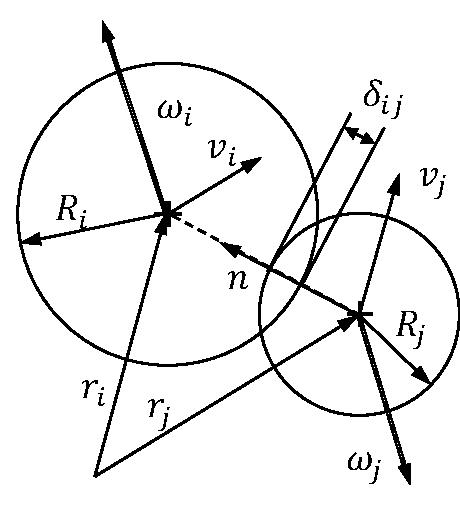
\includegraphics[scale=0.8]{collision.pdf}
  \centering
  \caption{Particle collision layout with the length of overlap $\delta$.}
  \label{fig:collision}
\end{figure}\vspace*{3pt}
The interaction force $F_i$ and torque $T_i$ in \equref{eq:restrictionDEM_EOM} can be determined using the collision model
\begin{flalign} \label{DEM_interactions}
&F_i=\sum_{j}{\left(F^n_{ij}+F^t_{ij}\right)} \\
&T_i=\sum_{j}{T_{ij}}
\end{flalign} itself
with $F_{ij}^n$ and $F_{ij}^t$ being the normal and tangential forces and $T_{ij}$ is the torque acting from particle $j$ to $i$.
\myparagraph{Normal contact force model}
The abovementioned overlapping length anneals the collision response of rigid objects by the $\delta$-dependent repulsive normal contact force model based on the Hertzian stress and damping
\begin{flalign} \label{DEM_normal_force}
&F_{ij}^n=(k_{Hz}\delta^{3/2}+c_{Hz}\delta^{1/4}\dot{\delta})n, \\
\end{flalign}
where
\begin{align} \label{DEM_Hertzian_spring}
&k_{Hz} = \frac{4}{3}\sqrt{R'}E', \\
&c_{Hz} = \frac{\sqrt{m'k_{Hz}}}{8} \\
\end{align}
are the spring and damping coefficients of the collision in normal direction with the effective quantities
\begin{align}
&R'=\frac{R_iR_j}{R_i+R_j}, \\
&m'=\frac{m_im_j}{m_i+m_j}, \\
&E'=\frac{E_iE_j}{E_j(1-\nu_i^2)+E_i(1-\nu_j^2)}.
\end{align}

\myparagraph{Tangential contact force and torque model}
The tangential or shear forces between colliding particles are determined by the relative linear and angular velocities $v_{ij}$ and $\omega_{ij}$. The tangential contact force model is written as
\begin{flalign} \label{DEM_tangential_force}
&F_{ij}^t=\min(k^tv^t,k^fF_{ij}^n),
\end{flalign}
where $k^v$ and $k^f$ are the tangential viscous damping and Coulomb friction coefficients respectively and
\begin{flalign} \label{DEM_tangential_velocity}
&v^t=v_{ij}-(v_{ij}n)n+R_i'n\times\omega_i+R_j'n\times\omega_j,
\end{flalign}
is the relative tangential velocity denoting the actual distance of particle $i$ and the contact point with $R_i'=(R_i-\delta/2)$. Finally, the tangential contact forces are used to calculate the resultant torque of particle $i$:
\begin{flalign} \label{DEM_tangential_force}
&T_i=\sum_j{R_i'n\times F_{ij}^t}.
\end{flalign}
Note that particle interaction forces and torques are calculated only when $\delta>0$, otherwise, the particles $i$ and $j$ are not in interaction with each other. The equations \equref{eq:restrictionDEM_EOM} form a system of $N$ algebraic equations that can be solved explicitly.\\


\subsubsection{Discrete Vortex Method (DVM)}
Vortex methods are meshless numerical tools for modelling inviscid fluid flow governed by point vortices. The basic idea behind vortex methods is that vorticity is a conserved quantity in inviscid flows, consequently the flow field can be determined using a set of point vortices drifting in the velocity field induced by them.
First of all the vorticity is defied as the curl of the velocity field $v$:
\begin{flalign} \label{DVM_vorticity}
&\omega=\nabla\times v.
\end{flalign}
For incompressible fluids the continuity equation reduces to
\begin{flalign} \label{DVM_continuity}
&\nabla\dot v=0,
\end{flalign}
which can be automatically satisfied by introducing the vector streamfunction such that
\begin{flalign} \label{DVM_vector_streamfunction}
&v=\nabla\times\Psi.
\end{flalign}
By assuming the vector streamfunction to be divergence free, the vorticity can now be expressed as
\begin{flalign} \label{DVM_vector_poisson}
&\omega\nabla\times\nabla\times\Psi=\nabla(\nabla\dot\Psi)-\nabla^2\Psi=-\nabla^2\Psi,
\end{flalign}
the vector Poisson's equation for the streamfunction. The equation \equref{DVM_vector_poisson} in case of a single point vortex at position $r_0$ with vorticity strength $\omega$ in infinite domain has the form
\begin{flalign} \label{DVM_poisson_single}
\nabla^2\Psi=-\omega\frac{\delta(|r-r_0|)}{2\pi |r-r_0|},
\end{flalign}
The solution of \equref{DVM_poisson_single} can be obtained by Green's function:
\begin{flalign} \label{DVM_streamfunction_single}
\Psi(r)=-\omega(r_0)\frac{ln|r-r_0|}{2\pi}.
\end{flalign}
The corresponding velocity field is calculated by
\begin{flalign} \label{DVM_velocity_single}
v(r)=\nabla\times\Psi=\frac{\omega\times (r-r_0)}{2\pi |r-r_0|^2}.
\end{flalign}
Considering the linearity of \equref{DVM_poisson_single} one can calculate the flow field induced by multiple vortex points by simply summing up the contributions of the individual vortices:
\begin{flalign} \label{DVM_velocity_multi}
v(r)=\sum_i\frac{\omega_i\times (r-r_i)}{2\pi |r-r_i|^2}.
\end{flalign}
The implication of point vortices may cause stability problems due to the singular velocity field at the point vortices. To circumvent such condition it is required to use vortex blobs instead of point vortices. A second order Gaussian approximation of the velocity in \equref{DVM_velocity_multi} is written as:
\begin{flalign} \label{DVM_velocity_multi_blob}
v(r)=\sum_i\frac{\omega_i\times (r-r_i)}{2\pi |r-r_i|^2}(1-e^{-r^2/\epsilon^2}),
\end{flalign}
where $\epsilon$ is the width of the Gaussian kernel. This approximation eliminates the numerically unmanageable high velocities in the immediate vicinity of vortex points but provides accurate velocity contribution elsewhere. The associated velocity field advects the vortex points in space without changing their strength of vorticity. Obviously the new layout of vortex points induces a different velocity field providing the subsequent instant of the time-dependent inviscid flow. Although there are several variants of vortex methods involving boundary conditions as constaints analogously to the Methods of Fundamental Solutions (MFS), only the basic Discrete Vortex Method is implemented in Nauticle.

\subsection{Temporal integration}
Numerical schemes for integration are required to solve time-dependent differential equations. Two numerical schemes are implemented in Nauticle.
\subsubsection{Explicit-Euler method}
This is a one-step explicit method to advance quantities in time by the
\begin{flalign}
\phi^{n+1}=\phi^n+\Delta t f(\phi^n,t^n)
\end{flalign}
expression, where $\phi$ is an arbitrary quantity, $f(\phi^n,t^n)$ is a function of $\phi$ and time $t$ in the $n$th time instant, and $\Delta t=t^{n+1}-t^n$ is the time step size.
\subsubsection{Second-order Runge-Kutta method}
The second order explicit Runge-Kutta or midpoint scheme consists of two integration steps. The first one is the prediction step
\begin{flalign}
\phi^{n+1/2}=\phi^n+\frac{\Delta t}{2} f(\phi^n,t^n),
\end{flalign}
which is followed by the evaluation of $f(\phi^{n+1/2},t^{n+1/2})$. The second step is the correction step to obtain the final value $\phi^{n+1}$:
\begin{flalign}
\phi^{n+1}=\phi^n+\Delta t f(\phi^{n+1/2},t^{n+1/2}).
\end{flalign}


\section{Implementation}
\subsection{The Nauticle environment} \label{sec:environment}
The basic idea of the Nauticle environment is that any particle method (regardless of the classification in Section \ref{sec:particle_method_classification}) can be considered as the determination of interactions between spatially distributed point-like nodes (particles). This assumption leads to the general interpretation of particle methods as \textit{interactions}. 

In this section the definitions corresponding to Nauticle are introduced, then the most important implementation methodologies and features of the solver are discussed.
\subsubsection{Definitions}
\textbf{Tensor}: Tensors in Nauticle have a few restrictions that are discussed here for the sake of clarity and simplicity. The tensor $T$ is a zeroth ($T\in\R$), first ($T\in\R^d$), or second ($T\in\R\otimes\R$) order real valued tensor, in $d=1,2,3$ dimensions. Throughout this guide tensors are considered to obey these restrictions, otherwise it is indicated. Furthermore, all the quantities (scalar, vector and tensor) are represented by tensors.

\textbf{Domain}: Consider the simply connected rectangular subset $\Gamma^d\subset\R^d$ ($d=1,2,3$), with edge size $\lambda\in\R$ and its boundary $\partial\Gamma^d$. The $\Gamma^d$ subset is a $d$ dimensional domain, if the
\begin{flalign}
\begin{split}
&1.\quad \Gamma^d=[r_{min},r_{max}] \puretext{such that} r_{min}<r_{max} \puretext{and} \{r_{min},r_{max}\} \in \R^d\\
&2.\quad \partial\Gamma^d=\bigcup_{d}{(r_{min}\cup r_{max})} \\
&3.\quad \lambda=r_{max}-r_{min}
\end{split}
\end{flalign}
conditions are satisfied.

\textbf{Particle}: A point-like object with position $r\in\Gamma^d$.

\textbf{Particle system}: The $P_{N}=\left\{r_i|i=1,2,...,N\right\}$ set of particles $r_i\in\Gamma^d$ is defined as a particle system of domain $\Gamma^d$.

\textbf{Field}: Consider a particle system $P_N$ of particles $r_i$, $i=1,2..N$. The set $F_N=\left\{f_i\leftarrow r_i \vert i=1,2,...,N\right\}$ is a field over $P_N$ if $f_i$ is a real valued zeroth, first or second order tensor associated to particle $i$.

\subsection{n-nearest neighbour search} \label{sec:neighbour_search}
One of the specific properties of particle methods is the continually changing particle layout. Since no interparticle structure is considered, the connectivity may change (except for Lagrangian or unbounded mollifier functions) with the particle positions. The naive ($N^2$ complexity) determination of particle interactions is usually unsatisfactory due to its high performance requirement, therefore a more efficient neighbour searching algorithm should be used instead. Here a simple and memory-efficient algorithm is implemented. The basic idea of the method is that a so-called hash key is assigned to each particle depending on the cell it occupies. Since all the particles that occupy the same cell obtain identical hash keys, the list of particles of the adjacent cells can be constructed easily.

The bottleneck of this algorithm is that the particle positions need to be sorted by the hash keys, which can be compuationally expensive. However, when the particle layout does not change too much before the recalculation of the hash keys, the sorting process is cheap because most of the particle's hash keys are already organised in the proper order.\\
\begin{figure}[h!]
  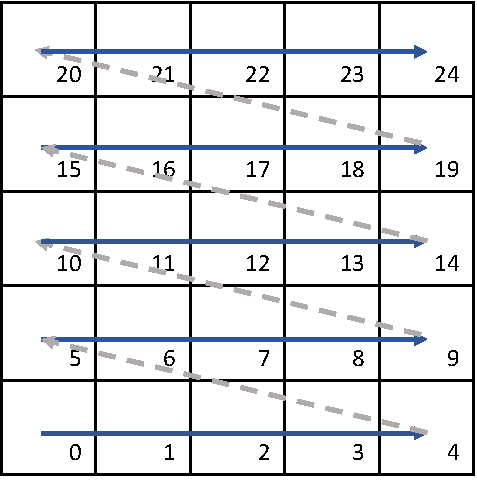
\includegraphics[scale=0.6]{hash_key.pdf}
  \centering
  \caption{Unfolding the two-dimensional domain to one dimension. The same procedure can be applied in three dimensions.}
  \label{fig:unfolding}
\end{figure}\vspace*{3pt}
\begin{figure}[h!]
  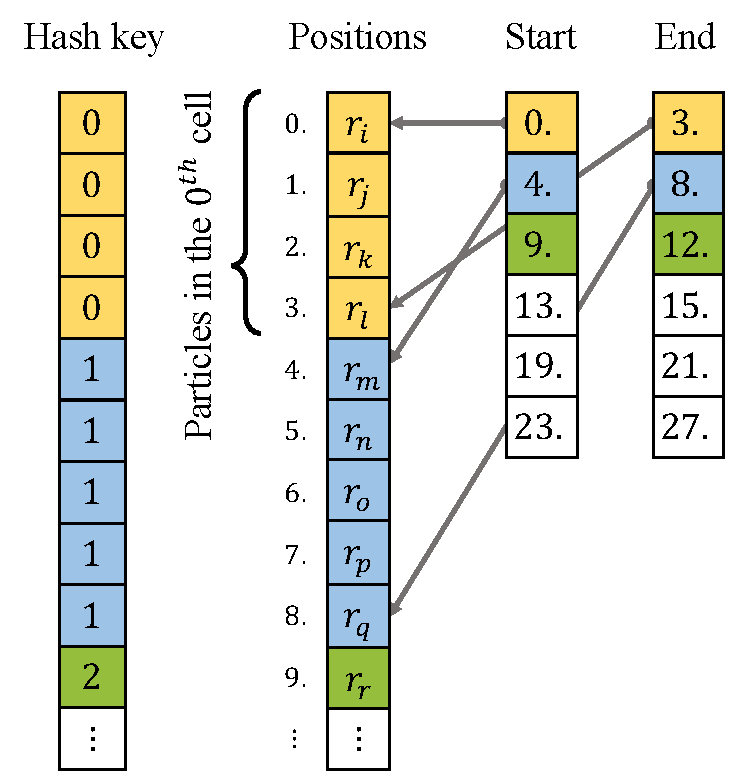
\includegraphics[scale=0.6]{nnsearch.pdf}
  \centering
  \caption{Indexing particle positions with Start and End arrays.}
  \label{fig:nnsearch}
\end{figure}\vspace*{3pt}

To determine interparticle connectivity the following steps are performed in Nauticle:
\begin{enumerate}
  \item Calculation of a hash key for each particle using the unfolding of the domain shown by Figure \ref{fig:unfolding},
  \item Sorting particles and the fields by the array of hash keys,
  \item Generating Start and End arrays containing the index of the first and last particle of each cell. The Start and End arrays are introduced in Figure \ref{fig:nnsearch}.
\end{enumerate}
Later, during the calculation of particle interactions, the particles of the adjacent cells of each particle are checked using the start and end arrays to mark the potential neighbours. Finally, the actual neighbours are calculated based on the set of potential neighbours. Due to computational optimisation, the steps above are not performed until the particle layout is changed.

\subsection{Periodic and symmetric boundaries}
The computational domain $\Omega$ defined in (TODO) forms the particles' frame of reference. Since no particle can ever exist outside the domain, the bounding surface $\partial\Omega$ applies symmetric or periodic rules to avoid the exclusion by handling particles that intend to cross the surface. Obviously, the opposite boundaries of $\Omega$ have to be both symmetric or periodic boundaries.
Both conditions imply the repositioning of exiting particle $i$ applying the
\begin{flalign} \label{eq:restriction}
r_i\leftarrow r_i mod \lambda
\end{flalign}
restriction, where $\lambda$ is the size of $\Omega$. However, exiting should ideally never occur in case of symmetric boundary. The restriction \equref{eq:restriction} does not provide either correct periodic or symmetric boundary conditions in itself. To take these conditions into account, the overhanging influence radius should be replaced or reflected properly. The physical interpretation of influence radius in the vicinity of periodic ($\partial\Omega_p$) and symmetric ($\partial\Omega_s$) boundaries is shown in Figure \ref{fig:periodic_symmetric}.
\begin{figure}
  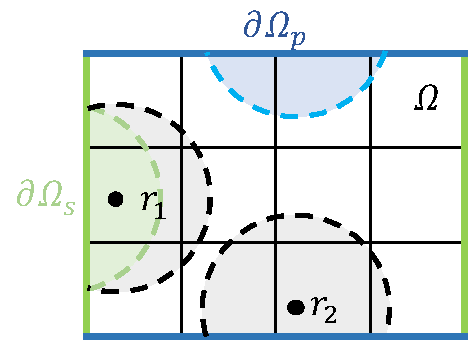
\includegraphics[scale=0.8]{periodic_symmetric_2.pdf}
  \centering
  \caption{ Shifting (blue) and reflecting (green) influence radius in the vicinity of periodic and symmetric boundary conditions respectively.}
  \label{fig:periodic_symmetric}
\end{figure}\vspace*{3pt}
During the calculation of interparticle distance vector $r_{ji}=r_j-r_i$ at the boundary the ensemble formula
\begin{flalign} \label{eq:boundary_interparticle_distance}
&r_{ji}=r_{ji}+\beta\delta(\delta-1)(r_{max}-r_j)+\beta\delta(\delta+1)(r_{min}-r_j)+(\beta-1)\floor{\frac{r_{ji}-r_{min}}{\lambda}}\lambda
\end{flalign}
is applied, where $\beta=0$ or $1$ for periodic or symmetric boundaries respectively, $\lambda$ is the size of $\Omega$, the operator $\floor{\cdot}$ denotes floor, $\delta$ is given by
\begin{flalign} \label{eq:delta_perioic_symmetric}
&\delta=-\floor{\frac{g_j-r_{min}}{N_c}},
\end{flalign}
with $g_j$ being the grid coordinate of particle $j$ and $N_c$ denotes the number of cells along the edges of $\Omega$. The grid coordinates of the adjacent particles is calculated by
\begin{flalign} \label{eq:grid_position_periodic_symmetric}
&g_j\leftarrow g_j+\delta(N_c-\beta N_c+\beta).
\end{flalign}
Since in case of the symmetric condition the interactions are calculated by particle mirroring, the vector and tensor quantities should be reflected using the reflection matrix
\begin{flalign} \label{eq:reflection_periodic_symmetric}
&R=I^d(-2\beta_i+1)^T,
\end{flalign}
where $I^d$ is a $d$ dimensional identity tensor. Note that in one dimension ($d=1$), it is required to distinguish scalars and single element vectors, because only scalar quantities should remain the same after reflection.



\subsection{Expression tree}
The generality of the numerical solver requires the analysis of user-defined expressions and equations (see Section \ref{UDE}). In Nauticle the expression parsing is based on the expression tree shown in Figure \ref{fig:expression_tree}.
\begin{figure}[h!]
  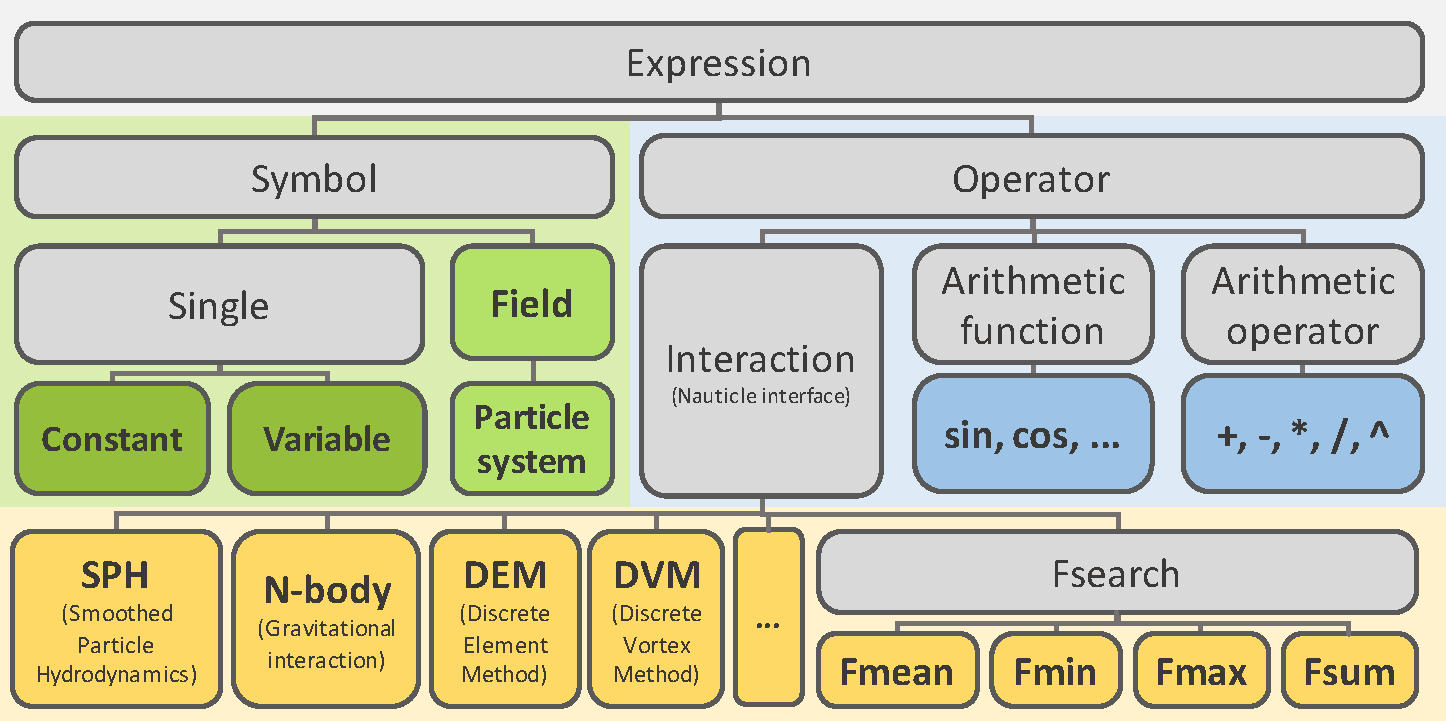
\includegraphics[scale=0.5]{expression_tree.pdf}
  \centering
  \caption{Expression tree: hierarchy of expression elements. The gray nodes in the tree indicate abstract types.}
  \label{fig:expression_tree}
\end{figure}\vspace*{3pt}

After the transformation of a user-defined expression to Reverse Polish Notation (RPN), the nodes of the expression tree can be employed to interpret the expresssion and perform its solution recursively. A simple example is presented by Figure \ref{fig:expression_example}.
\begin{figure}[h]
  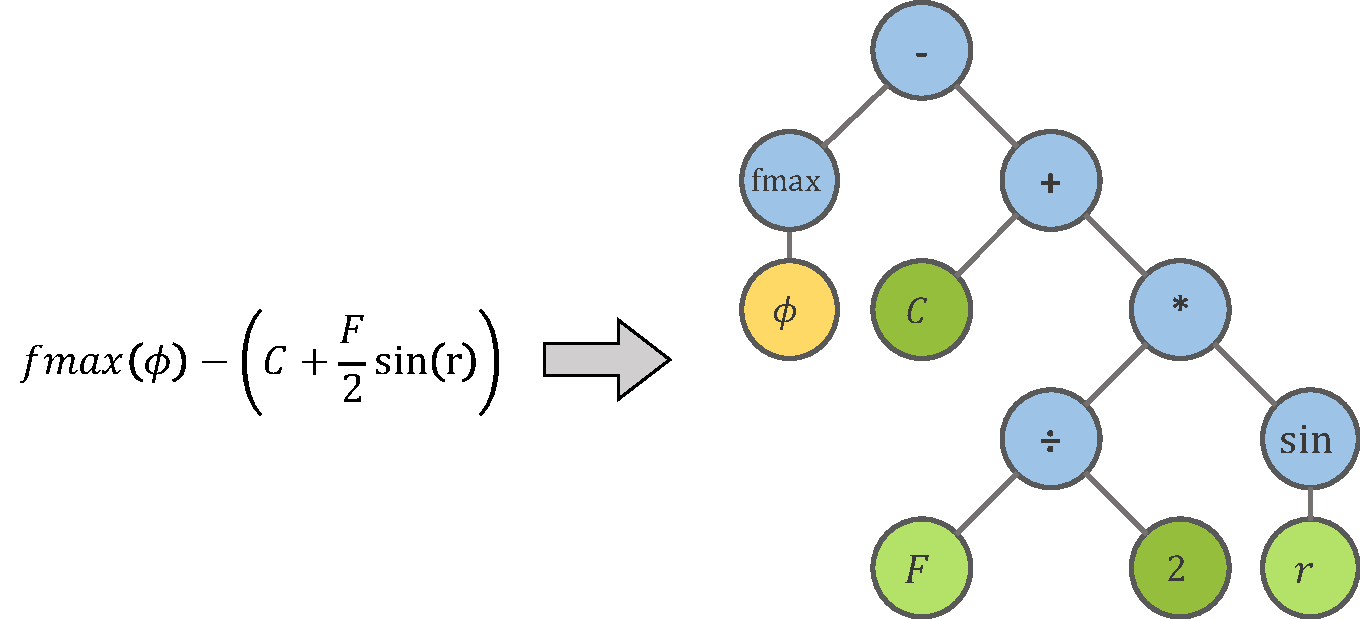
\includegraphics[scale=0.5]{expression_example.pdf}
  \centering
  \caption{Example for construction of expressions using the nodes of the expression tree.}
  \label{fig:expression_example}
\end{figure}\vspace*{3pt}

Although the nodes of the expression tree implement different quantities and operators of Nauticle, all nodes are considered as tensors. In the following, the branches and nodes of the expression tree are discussed.

\subsubsection{The symbol branch}
On the one hand, the single symbols like constants and variables represent global values for the simulation (such as the time step size or gravitational acceleration), which usually have the same value for each particle, consequently one (single) instance is sufficient to be stored. Therefore the single quantities have very small memory requirements. However, in case of multistep integrators, the desired number of former values of variables are automatically stored. Obviously it is unnecessary for constant values, since they cannot be changed during their lifetime. On the other hand, the fields are interpreted over a set of spatial nodes (particles) storing tensor values assigned to each of the particles. Former values for multistep integrators are automatically stored as well, as in case of the variables. A special implementation of a field is the particle system itself, storing the particle positions as field variables. The particle system is special not only because it stores particle positions but it performs n-nearest neighour search and stores the computational domain too. The restriction of particles to the domain is also performed by the particle system.

\subsubsection{The operator branch}
The other main branch of the expression tree is the branch of operators acting on symbols. Operators are classified into three groups:
\begin{itemize}
  \item Arithmetic operators,
  \item Arithmetic functions,
  \item Interactions.
\end{itemize}
The first two groups of operators evaluate operations on single quantities or particlewise field quantities (e.g. addition of two fields), while the interactions require field data (e.g. value of field maximum or minimum).
\myparagraph{Arithmetic operators}
The supported arithmetic operators are presented in Table \ref{tbl:arop}.
\begin{table}
\begin{center}
\caption{Supported arithmetic operators in Nauticle.}\label{tbl:arop}
\begin{tabular}{ l c c c c }
\toprule[1.5pt]
\bf Operator name & \bf Sign & \bf Operands & \bf Description\\ 
\midrule
Addition & "+" & 2 & $[n \times m] + [n \times m]$\\ 
Subtraction & "-" & 2 & $[n \times m] - [n \times m]$\\ 
Product & "*" & 2 & $[n \times m] * [m \times n]$\\ 
Term by term product & ":" & 2 & $[n \times m] : [n \times m]$\\ 
Power & "$\hat{\ }$" & 2 & $[n \times m] \hat{\ } [1 \times 1]$\\ 
Positive & "+" & 1 & $[n \times m]$\\ 
Negative & "-" & 1 & $[n \times m]$\\ 
\bottomrule[1.25pt]
\end{tabular}
\end{center}
\end{table}
The arithmetic operators are valid for tensors with conforming sizes (last column of Table \ref{tbl:arop}).
\myparagraph{Arithmetic functions}
The arithmetic functions supported by Nauticle are summarised in Table \ref{tbl:arfc}. It should be noted here that complex numbers are currently not supported by the tensor implementation, therefore some of the functions may give uninterpretable results (e.g. $\sqrt{-1}$ is not a number in Nauticle).
\begin{table}
\begin{center}
\caption{Supported arithmetic functions in Nauticle.}\label{tbl:arfc}
\begin{tabular}{ l l c | l l c }
\toprule[1.5pt]
\bf Funcion & \bf Name & \bf Op's & \bf Funcion & \bf Name & \bf Op's\\ 
\midrule
Absolute value & $abs$ & 1 & Modulo & $mod$ & 2 \\
Arc cosine & $acos$ & 1 & Random in range & $rand$ & 2 \\
Arc co-tangent & $acot$ & 1 & Sign & $sgn$ & 1 \\
Arc sine & $asin$ & 1 & Sine & $sin$ & 1 \\
Arc tangent & $atan$ & 1 & Sine hyperbolic & $sinh$ & 1 \\
Cosine & $cos$ & 1 & Square root & $sqrt$ & 1 \\
Cosine hyperbolic & $cosh$ & 1 & Tangent & $tan$ & 1 \\
Co-tangent & $cot$ & 1 & Tangent hyperbolic & $tanh$ & 1 \\
Co-tangent hyperbolic & $coth$ & 1 & Trace & $trace$ & 1 \\
Cross product & $cross$ & 2 & Tanspose & $transpose$ & 1 \\
Exponential & $exp$ & 1 & Trunc & $trunc$ & 1 \\
Floor & $floor$ & 1 & Matrix determinant & $determinant$ & 1 \\
Greater than & $gt$ & 2 & Matrix inverse & $inverse$ & 1 \\
Natural logarithm & $log$ & 1 & Equal & $eq$ & 2 \\
Less than & $lt$ & 2 & Logical and & $and$ & 2 \\
Vector lenght & $magnitude$ & 1 & Logical or & $or$ & 2 \\
Maximum & $max$ & 2 & Logical negation & $not$ & 1 \\
Minimum & $min$ & 2 & Logical exclusive or & $xor$ & 2 \\
Tensor element & $elem$ & 3 & Logical condition & $if$ & 3 \\
\bottomrule[1.25pt]
\end{tabular}
\end{center}
\end{table}

\myparagraph{Interactions}
It was pointed out earlier in Section \ref{sec:environment} that any particle method can be considered as a collection of particle interaction laws. Accordingly, the interaction branch forms an essential part of not only the expression tree but also the Nauticle environment. This group of operators deals with particle interactions that certainly depend on field quantities (and the particle system). Furthermore the interaction branch provides an intermediate development interface, which is introduced in detail later in Section \ref{sec:interface}.
The simplest functions in this branch are presented in Table \ref{tbl:fsearch}. Since the magnitude of an arbitrary tensor quantity is ambiguous, these field-functions can be evaluated only over scalar fields (last column of Table \ref{tbl:fsearch}). These functions have linear computational complexity.
\begin{table}
\begin{center}
\caption{Simple interaction operators.}\label{tbl:fsearch}
\begin{tabular}{ l l c c }
\toprule[1.5pt]
\bf Operator & \bf Name & \bf Operands & \bf Description\\
\midrule
Field maximum & $fmax$ & 1 & $[1 \times 1]$\\ 
Field minimum & $fmin$ & 1 & $[1 \times 1]$\\ 
Field average & $fmean$ & 1 & $[1 \times 1]$\\
\bottomrule[1.25pt]
\end{tabular}
\end{center}
\end{table}
Further interaction operators in Nauticle belong to the particle methods presented in Section \ref{sec:implemented}.

\section{Using Nauticle}
\subsection{Simulation workflow} \label{sec:sim_workflow}
To define and simulate a problem a form (XML-document) is needed to be passed to the solver. The form contains all the required information about the physical model called case. In this section the structure of the form is discussed through the introduction of the workspace and the user-defined equations.
\subsubsection{Definitions}
\textbf{Workspace}: A collection of user-defined symbols like constants, variables, fields and particle system representing the quantities of the physical model.

\textbf{User-defined equation (UDE)}: Equation, built up using the nodes of the expression tree and the objects stored in the workspace. The evaluation of an equation means the assignment of the RHS solution to the LHS. Consequently the LHS should be a variable, field or particle system. Each UDE has a condition with a default value "true" that determines if the equation has to be solved or not. The condition may have particle-dependent value.

\textbf{Parameter space}: An object to hold information about the solution data export.

\begin{figure}[h!]
  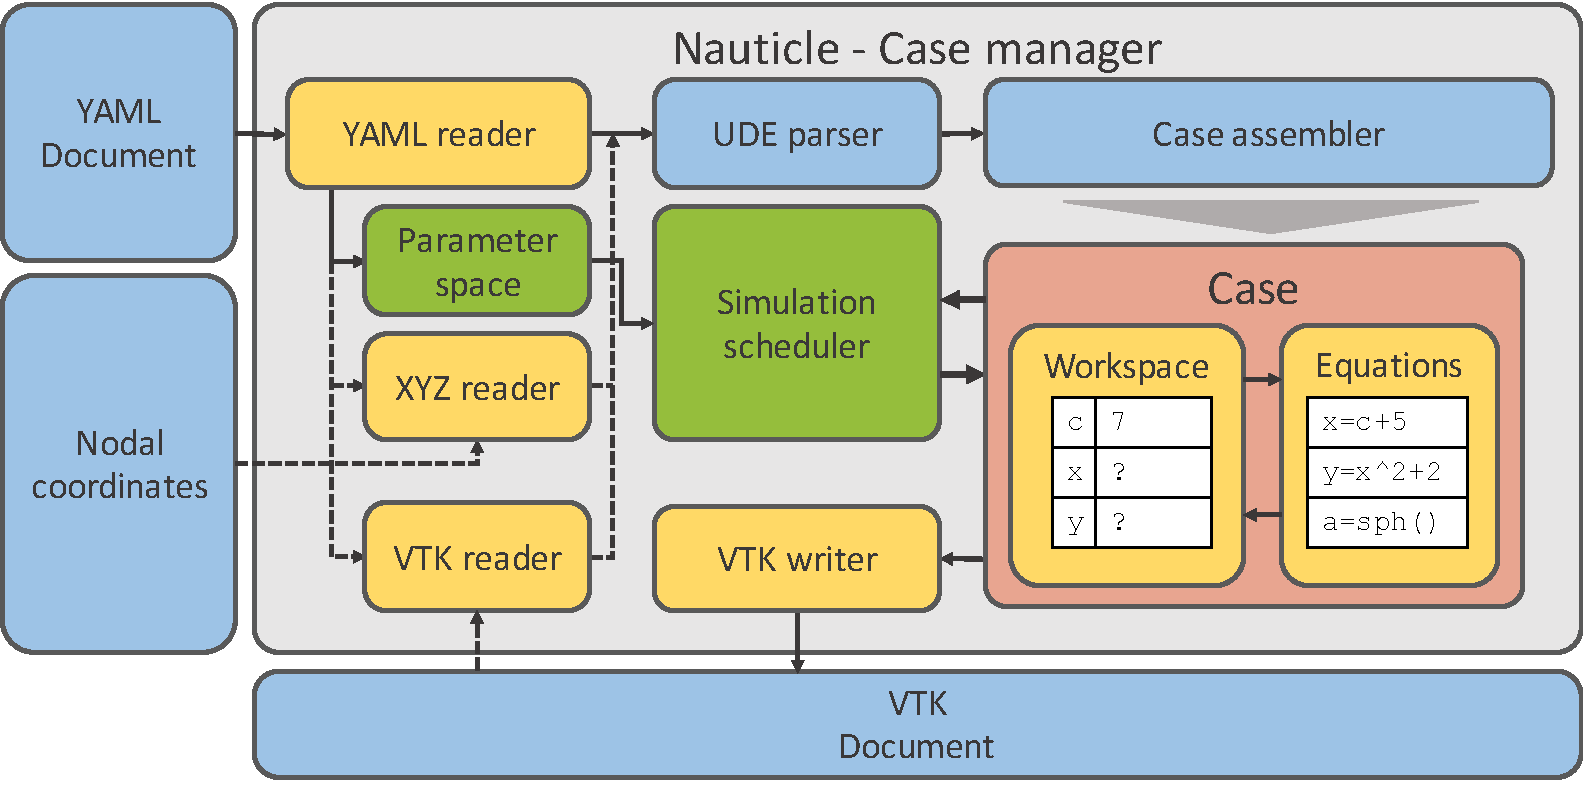
\includegraphics[scale=0.55]{workflow.pdf}
  \centering
  \caption{Outline of the simulation flow.}
  \label{fig:workflow}
\end{figure}\vspace*{3pt}

The schematic diagram of a simulation is presented in Figure \ref{fig:workflow}. After the parsing of the input files on the left, the case assembler builds the case, which is handled by the simulation scheduler. The latter is responsible for the calculation flow and parallelisation. The result files are saved by the VTK-writer governed by the case manager. 
As soon as the simulation scheduler sends a step request, the solution of the UDE's is carried out by the case itself. The change of the value of any symbol contained by the workspace during the solution is automatically updated. Optionally, any of the result files can be applied as initial conditions for a further simulation (see Section \ref{sec:XML}).

\subsection{Input/Output file formats}
During the execution of a simulation, Nauticle works with four types of input and output files. Some of these files are fundamental, the others are optional. The subsequent sections introduce these file types more or less in the order of importance.
\subsubsection{VTK-document}
VTK is a general purpose library for visualisation and storage of arbitrary geometry. To store simulation results, VTK formatted ASCII or binary files are used.
\myparagraph{Simple Legacy Formats}
The legacy VTK file formats consist of five basic parts.
\begin{itemize}
\item 1. The first part is the file version and identifier. This part contains the single line: \# vtk DataFile Version x.x. This line must be exactly as shown with the exception of the version number x.x, which will vary with different releases of VTK. (Note: Nauticle supports version 4.0) 
\item 2. The second part is the header. The header consists of a character string terminated by end-of-line character. The header is 256 characters maximum. The header can be used to describe the data and include any other pertinent information. 
\item 3. The next part is the file format. The file format describes the type of file, either ASCII or binary. On this line the single word ASCII or BINARY must appear. 
\item 4. The fourth part is the dataset structure. The geometry part describes the geometry and topology of the dataset. This part begins with a line containing the keyword DATASET followed by a keyword describing the type of dataset. Then, depending upon the type of dataset, other keyword/ data combinations define the actual data.
\item 5. The final part describes the dataset attributes. This part begins with the keywords POINT\_DATA or CELL\_DATA, followed by an integer number specifying the number of points or cells, respectively. (It doesn't matter whether POINT\_DATA or CELL\_DATA comes first.) Other keyword/ data combinations then define the actual dataset attribute values (i.e. scalars, vectors, tensors, normals, texture coordinates, or field data). 
\end{itemize}
In Nauticle the result files contain the whole case including the workspace and UDE's. The DATASET type is POLYDATA, while the symbols and UDE's are stored as string formatted data.
\subsubsection{XML-document} \label{sec:XML}
The XML-document is the most important and fundamental input file of any simulation executed by Nauticle. No simulation can be executed in absense of the configuration XML-file. Nevertheless, they can be distinguished by the data they contain. The most important advantage of the application of XML-files is that they support random access to the stored data, therefore the user is not required to follow strict rules during the construction of the simulation problem.
\begin{figure}[h!]
  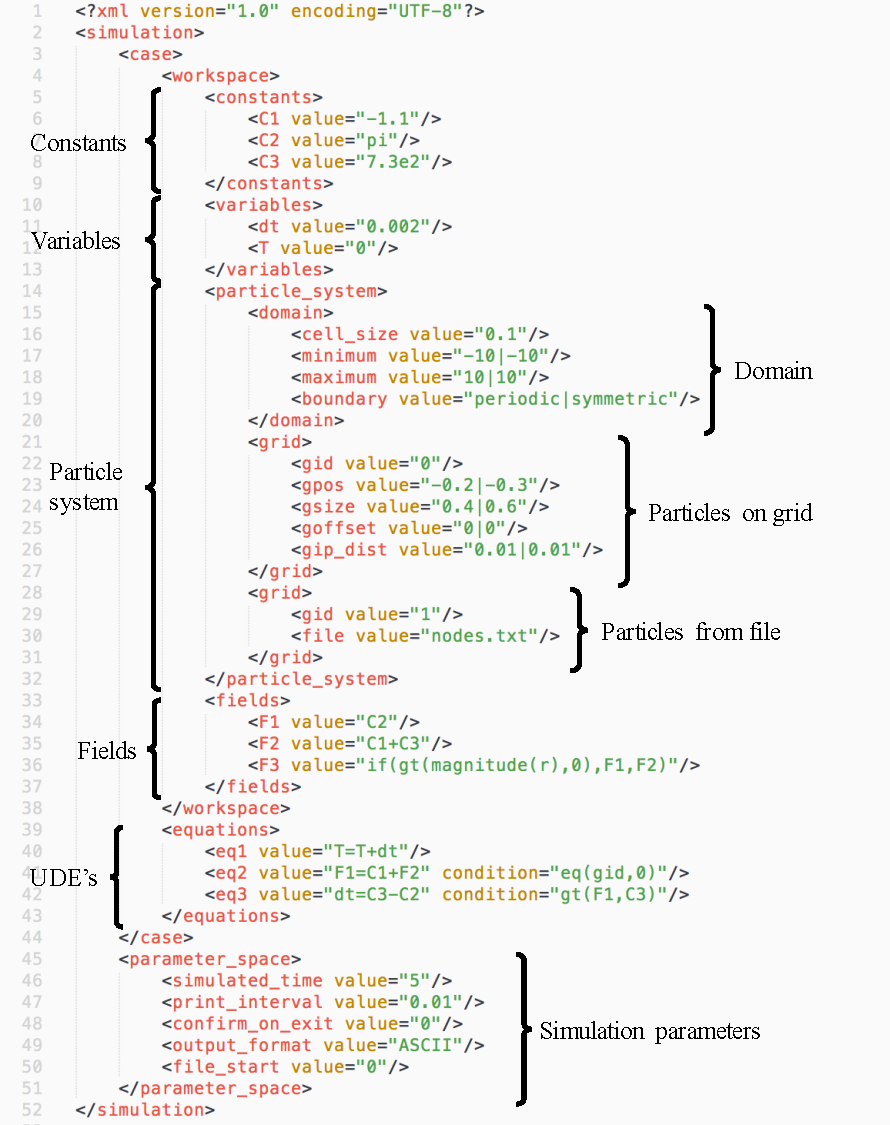
\includegraphics[scale=1.05]{xml_intro.pdf}
  \centering
  \caption{Structure of the XML-document.}
  \label{fig:xml_intro}
\end{figure}\vspace*{3pt}
A simple document is presented in Figure \ref{fig:xml_intro}, in which the whole workspace and list of equations to be passed to the solver are defined and no external sources are used except for the nodal coordinates (which is optional). Another way of problem initialisation is the application of a former simulation result stored in VTK file. Despite of that, XML-documents cannot be omitted, but are used to refer to the desired input file. This type of initialisation allows a significantly simpler XML-document as it is illustrated in Figure \ref{fig:xml_intro_simple}.
\begin{figure}[h!]
  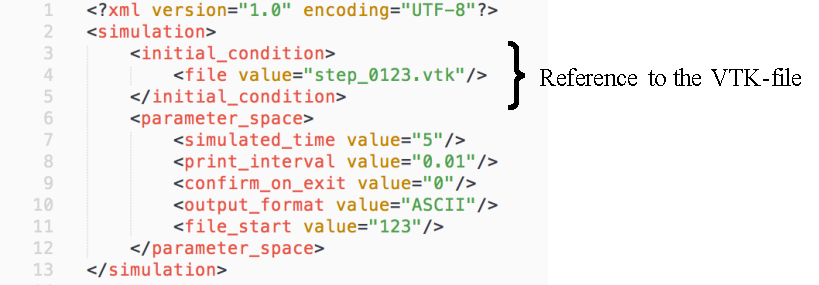
\includegraphics[scale=1]{xml_intro_simple.pdf}
  \centering
  \caption{Structure of the XML-document referring to a former simulation result.}
  \label{fig:xml_intro_simple}
\end{figure}\vspace*{3pt}
\newpage
Note that in this configuration the workspace and list of equations are also stored in the VTK file:\\
\begin{lstlisting}
# vtk DataFile Version 4.0
vtk output
ASCII
DATASET POLYDATA
FIELD FieldData 4
domain 1 4 string
domain_min:-10|-10
domain_max:10|10
cell_size:0.1
boundary:0|1
variables 1 2 string
dt:0.002
T:0
constants 1 3 string
C1:-1.1
C2:3.14159
C3:730
equations 1 3 string
eq1:T=(T+dt)#1
eq2:F1=(C1+F2)#eq(gid,0)
eq3:dt=(C3-C2)#gt(F1,C3)
...
\end{lstlisting}
The character "\#" marks the solution condition for each UDE.
\subsubsection{Text document}
The particle cloud can be optionally defined through text files containing the set of nodal positions instead of the uniform grid generation based on the XML data. Note that the text file should always contain three-dimensional coordinates separated by spaces or tabs. The dimensions of the problem are then defined by the domain and only the relevant coordinates of the nodal positions are considered, other coordinates are dropped.
\subsubsection{Log files}
The simulation log file contains the simulation data as it appears in terminal during runtime. Each execution produces a single log file with the name "sim.log" by default. A previous log file with the same name in the working directory is purged at the beginning of the calculation without approval.
\subsection{Runtime commands}
There are further optional commands that cannot be defined in the XML-document. These are the runtime commands summarised in Table \ref{tbl:runtime_commands}. To obtain information about the reserved names you need to use the "-wsres" command. Nauticle offers parallelisation on multicore CPU systems. By default, the number of threads to use during the execution is the number of available threads. Hovewer, you may want to limit the solver by defining the actual number threads to use. This can be done by the "-numthreads N" command, where N is the desired number of threads. 
\begin{table} [h]
\begin{center}
\caption{Runtime commands.} \label{tbl:runtime_commands}
\begin{tabular}{ l l l }
\toprule[1.5pt]
\bf  & \bf Command & \bf Description\\
\midrule
1. & -help & Display Nauticle information. \\
2. & -wsres & Lists all reserved names in workspace. \\
3. & -numthreads <number> & Defines the number of threads to use. Default is detected. \\
4. & -xmlname <filename> & Defines the name of the XML input file. \\
5. & -logfile <filename> & Defines the name of the output log file. \\
6. & -wdir <directory> & Defines the working directory. Full path is required. \\
7. & -version & Prints the version number. \\
\bottomrule[1.25pt]
\end{tabular}
\end{center}
\end{table}















\section{Installation}
\subsection{Requirements}
Currently the installation process does not support Windows, it works only on Linux (distributions that support Application Package Tool (APT)) and Mac OSX systems. Hereinafter Linux is considered to support APT.
Nauticle requires a few dependencies and requirements to be installed. These are the following:
\begin{itemize}
  \item cmake (at least version 3.5) (\myhref{https://cmake.org/download/}{https://cmake.org/download/}),
  \item Visualization Toolkit 7.0.0 (\myhref{http://www.vtk.org/files/release/7.0/VTK-7.0.0.zip}{http://www.vtk.org/files/release/7.0/VTK-7.0.0.zip}),
  \item Common utilities (\href{https://bitbucket.org/BalazsToth/commonutils}{https://bitbucket.org/BalazsToth/commonutils}),
  \item ProLog (\myhref{https://bitbucket.org/BalazsToth/prolog}{https://bitbucket.org/BalazsToth/prolog}),
  \item HandyXML (\myhref{https://bitbucket.org/BalazsToth/handyxml}{https://bitbucket.org/BalazsToth/handyxml}).
\end{itemize}
The details of the required dependencies are not discussed here, please follow the links to find more information about the listed packages. Further dependencies could be required by the Visualization Toolkit.

During the installation process it is assumed that the user has internet connection and root privileges in the operating system (super user). Throughout the following subsection the automatic installation procedure is discussed in detail.
Note: to avoid any version conflicts it could be preferable to install and build Nauticle with its dependencies using HashDist, which is an environment management system (\myhref{https://github.com/hashdist/hashdist}{https://github.com/hashdist/ hashdist}). However it is not mandatory and the automated installation process does not apply HashDist.
\subsection{Automated installation}
Although it is possible to install and build the dependencies and Nauticle manually, it is recommended to use the installation shell script arriving with Nauticle. The script installs the whole package including the dependencies by typing the command
\begin{lstlisting}[language=bash]
  $ sh (*@\installer{}@*)
\end{lstlisting}
in terminal after changing directory to the desired folder. The content of the script with explanations is as follows:

\begin{example}{\installer{}}{}
\lstset{basicstyle=\tiny}
\begin{lstlisting}[language=bash]
#!/bin/sh

# Versions of nauticle and its dependencies
NAUTICLE_version="1.0.170221"
VTK_version="7.0.0"
CU_VERSION="1.0.170221"
PL_version="1.0.170221"
HX_version="1.0.170502"

# Set current directory to install directory.
INSTALL_DIR=$PWD
sudo chmod -R 777 ${INSTALL_DIR}

# Set OS variable (assume linux)
OS="Linux"
if [ "$(uname)" = "Darwin" ]; then
# if mac, install wget, and cmake
    brew install wget
    brew install cmake
    OS="Mac"
elif [ $OS = "Linux" ]; then
# if linux, install opengl and cmake
    sudo apt-get update
  sudo apt-get --yes --force-yes install build-essential
  sudo apt-get --yes --force-yes install freeglut3-dev
  sudo apt-get --yes --force-yes install cmake
fi

# Install proper version of VTK library
wget http://www.vtk.org/files/release/7.0/VTK-$VTK_version.zip
sudo unzip VTK-$VTK_version.zip -d /usr/local/
cd /usr/local/VTK-$VTK_version
sudo cmake .
sudo make

# Go to install directory
cd $INSTALL_DIR

# Download and unzip the required packages
# Common utils
wget https://bitbucket.org/nauticleproject/commonutils/downloads/commonutils-$CU_VERSION.zip
sudo unzip commonutils-$CU_VERSION.zip
sudo chmod -R 777 commonutils
rm commonutils-$CU_VERSION.zip
# Prolog
wget https://bitbucket.org/nauticleproject/prolog/downloads/prolog-$PL_version.zip
sudo unzip prolog-$PL_version.zip
sudo chmod -R 777 prolog
rm prolog-$PL_version.zip
# HandyXML
wget https://bitbucket.org/nauticleproject/handyxml/downloads/handyxml-$HX_version.zip
sudo unzip handyxml-$HX_version.zip
sudo chmod -R 777 handyxml
rm handyxml-$HX_version.zip
# nauticle
wget https://bitbucket.org/nauticleproject/nauticle/downloads/nauticle-$NAUTICLE_version.zip
sudo unzip nauticle-$NAUTICLE_version.zip
sudo chmod -R 777 nauticle
rm nauticle-$NAUTICLE_version.zip

# Install the dependencies and the nauticle executable (nauticle) itself
cd commonutils
sudo cmake .
sudo cmake .
sudo make install
cd ..
 
cd prolog
sudo cmake .
sudo cmake .
sudo make install
cd ..
 
cd handyxml
sudo cmake .
sudo cmake .
sudo make install
cd ..

# Set directory name for executable
BIN_DIR="${INSTALL_DIR}/nauticle/bin/$OS"
cd nauticle
sudo cmake .
sudo cmake .
sudo mkdir $BIN_DIR
sudo make
cd ..

# Add BIN_DIR to the environmental PATH variable
if [ "$OS" = "Mac" ]; then
  sudo printf "\nexport PATH=\${PATH}:$BIN_DIR\n" >> ~/.bash_profile
    alias brc='source ~/.bash_profile'
elif [ "$OS" = "Linux" ]; then
  sudo printf "\nexport PATH=\${PATH}:$BIN_DIR\n" >> ~/.bashrc
  alias brc='source ~/.bashrc'
fi

# Generate script file to run nauticle
# (this file is optional and probably useful only when using Nauticle through ssh)
sudo rm -f start.sh
sudo touch start.sh
sudo chmod 777 start.sh
printf "#!/bin/sh\nshift\nexecutable=$BIN_DIR/nauticle\n" >> start.sh
printf "sudo \$executable \"\$@\"" >> start.sh

\end{lstlisting}
\end{example}

It downloads and builds the necessary files in your system. After installation, the executable (\execname{}) will be placed in the bin directory and the \textbf{start.sh} file will be generated in the installation directory. The installer also adds the bin directory to your environment variables, therefore you can run it from different directories by simply typing \textbf{nauticle} in terminal. To activate this feature it may be necessary to manually reload the \textbf{.bash\_profile} or \textbf{.bashrc} file in your home directory using the \texttt{source} command.
In certain cases, when environment variables are not available you can perform computations using the \textbf{start.sh} file in the simulation folder:
\begin{lstlisting}[language=bash]
  $ sh start.sh
\end{lstlisting}
Note that the optional runtime commands are forwarded by \textbf{start.sh}, which supports the execution of
\begin{lstlisting}[language=bash]
  $ sh start.sh <arguments_list>
\end{lstlisting}
where the arguments\_list consists of the option listed in Table \ref{tbl:runtime_commands}.

\section{Nauticle interface} \label{sec:interface}

\section{Examples} \label{sec:examples}
\subsection{Couette-flow}
\subsubsection{Problem definition}
One of the simplest and most frequently investigated fundamental test case in fluid mechanics is the laminar Couette-flow. The upper one of the two infinite sized parallel walls shown in Figure \ref{fig:couette} is moving in $y$ direction with velocity $v=1$m/s.
\begin{figure}[h!]
  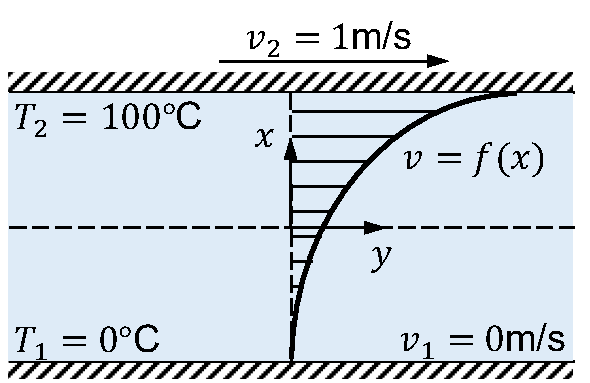
\includegraphics[scale=0.7]{couette.pdf}
  \centering
  \caption{Temperature-dependent laminar Couette-flow between parallel walls.}
  \label{fig:couette}
\end{figure}\vspace*{3pt}
The walls have different temperatures $T_1=0^\circ$C and $T_2=100^\circ$C affecting the fluid temperature and consequently the kinematic viscosity $\nu$ by the
\begin{equation}
\nu(T)=\nu_0 \exp(-bT)
\end{equation}
formula. The constants here are chosen to be $\nu_0=0.1\rm{m}^2/\rm s$ and $b=0.03 ^\circ C^{-1}$. Since the flow is laminar, the temperature distribution between the parallel walls can be determined by the heat equation
\begin{equation} \label{eq:couette_laplace}
\frac{\partial T}{\partial t}=\lambda\Delta T,
\end{equation}
where $\lambda=0.01$ is the heat conduction coefficient. The fluid velocity in the channel is governed by 
\begin{equation} \label{eq:couette_eom}
\frac{\partial v}{\partial t}=\nabla(\nu(T)\nabla v),
\end{equation}
where $v$ is the fluid velocity field. The problem is stationary and one-dimensional, therefore equations \equref{eq:couette_laplace} and \equref{eq:couette_eom} can be simplified as
\begin{flalign} \label{eq:couette_simplified}
\begin{split}
&\frac{d^2T}{dx^2}=0, \\
&\frac{d}{dx}\bigg(\nu(T)\frac{dv}{dx}\bigg)=0,
\end{split}
\end{flalign}
Applying Dirichlet boundary conditions for both the temperature and velocity fields:
\begin{flalign} \label{eq:couette_bc}
\begin{split}
&T(-L/2)=0,\\
&T(L/2)=100, \\
&v(-L/2)=0, \\
&v(L/2)=1, \\
\end{split}
\end{flalign}
where $L=1$m is the width of the channel, the solution of \equref{eq:couette_simplified} can be constructed analytically:
\begin{flalign} \label{eq:couette_analytical}
\begin{split}
&T(x)=\frac{T_2-T_1}{L}x+\frac{T_1+T_2}{2}=100x+50,\\
&v(x)=\frac{v_2-v_1}{e^{bT_1}-e^{bT_2}}(e^{bT(x)}-e^{bT_1})+v_1=\frac{e^{b(100x+50)}-1}{e^{100b}}.\\
\end{split}
\end{flalign}

\subsubsection{Numerical model and results}
To solve the Couette-flow problem the simplest model is built in Nauticle using the SPH collocation scheme. Although SPH is Lagrangian (particles should follow material trajectories), in the case of laminar parallel flow, the movement of particles can be omitted due to the identity of the Lagrangian and Eulerian fields. The time dependent discretised system of equations are
\begin{flalign} \label{eq:couette_sph_discretised}
\begin{split}
&\frac{dT_i}{dt}=\lambda\sum_j{2(T_j-T_i)\frac{1}{r_{ji}}\frac{m_j}{\rho_j}\nabla W_{ij}}, \\
&\frac{dv_i}{dt}=\sum_j{(\nu_j+\nu_i)(v_j-v_i)\frac{1}{r_{ji}}\frac{m_j}{\rho_j}\nabla W_{ij}}. \\
\end{split}
\end{flalign}
After the discretisation the XML-document can be constructed:
\begin{example}{Couette-flow configuration file}{}
\lstset{basicstyle=\tiny}
\begin{lstlisting}[language=XML]
<?xml version="1.0" encoding="UTF-8"?>
<simulation>
    <case>
        <workspace>
            <constants>
                <L value="1"/>
                <csize value="L/20"/>
                <dx value="csize/2"/>
                <rho0 value="1000"/>
                <mass value="dx*rho0"/>
                <lambda value="0.01"/>
                <nu0 value="0.1"/>
                <b value="0.03"/>
                <T1 value="0"/>
                <T2 value="100"/>
                <v1 value="0"/>
                <v2 value="1"/>
            </constants>
            <variables>
                <dt value="0.0025"/>
                <Time value="0"/>
            </variables>
            <particle_system>
                <domain>
                    <cell_size value="csize"/>
                    <minimum value="-L/csize/2-1"/>
                    <maximum value="L/csize/2+1"/>
                    <boundary value="periodic"/>
                </domain>
                <grid> <!-- bottom boundary particles -->
                    <gid value="1"/>
                    <gpos value="-L/2-csize+dx/2"/>
                    <gsize value="csize"/>
                    <goffset value="0"/>
                    <gip_dist value="dx"/>
                </grid>
                <grid> <!-- fluid particles -->
                    <gid value="0"/>
                    <gpos value="-L/2+dx/2"/>
                    <gsize value="L-dx"/>
                    <goffset value="0"/>
                    <gip_dist value="dx"/>
                </grid>
                <grid> <!-- top boundary particles -->
                    <gid value="2"/>
                    <gpos value="L/2-dx/2"/>
                    <gsize value="csize"/>
                    <goffset value="0"/>
                    <gip_dist value="dx"/>
                </grid>
            </particle_system>
            <fields>
                <a value="0"/>
                <v value="if(eq(0,gid),0,if(eq(gid,1),v1,v2))"/> <!-- initial condition -->
                <T value="if(eq(0,gid),0,if(eq(gid,1),T1,T2))"/> <!-- initial condition -->
                <T_dot value="0"/>
                <nu value="0.1"/>
            </fields>
        </workspace>
        <equations>
            <time value="Time=Time+dt"/>
            <heat value="T_dot=lambda*sph_L00(T,mass,rho0,Wp32210,csize)" condition="eq(gid,0)"/>
            <temp value="T=euler(T,T_dot,dt)" condition="eq(gid,0)"/>
            <viscosity value="nu=nu0*exp(-b*T)"/>
            <moment value="a=sph_L10(nu,v,mass,rho0,Wp32210,csize)" condition="eq(gid,0)"/>
            <vel value="v=euler(v,a,dt)" condition="eq(gid,0)"/>
        </equations>
    </case>
    <parameter_space>
        <simulated_time value="100"/>
        <print_interval value="1"/>
        <confirm_on_exit value="false"/>
        <output_format value="BINARY"/>
    </parameter_space>
</simulation>
\end{lstlisting}
\end{example}
Since the initial conditions of both the temperature and velocity are uniform, the solution of the discretised equations needs to be repeated until the result is sufficiently formed. In this case the simulated time is $100$s. The final result is compared with the analytical solution in Figure \ref{fig:couette_results}.
\begin{figure}[h!]
  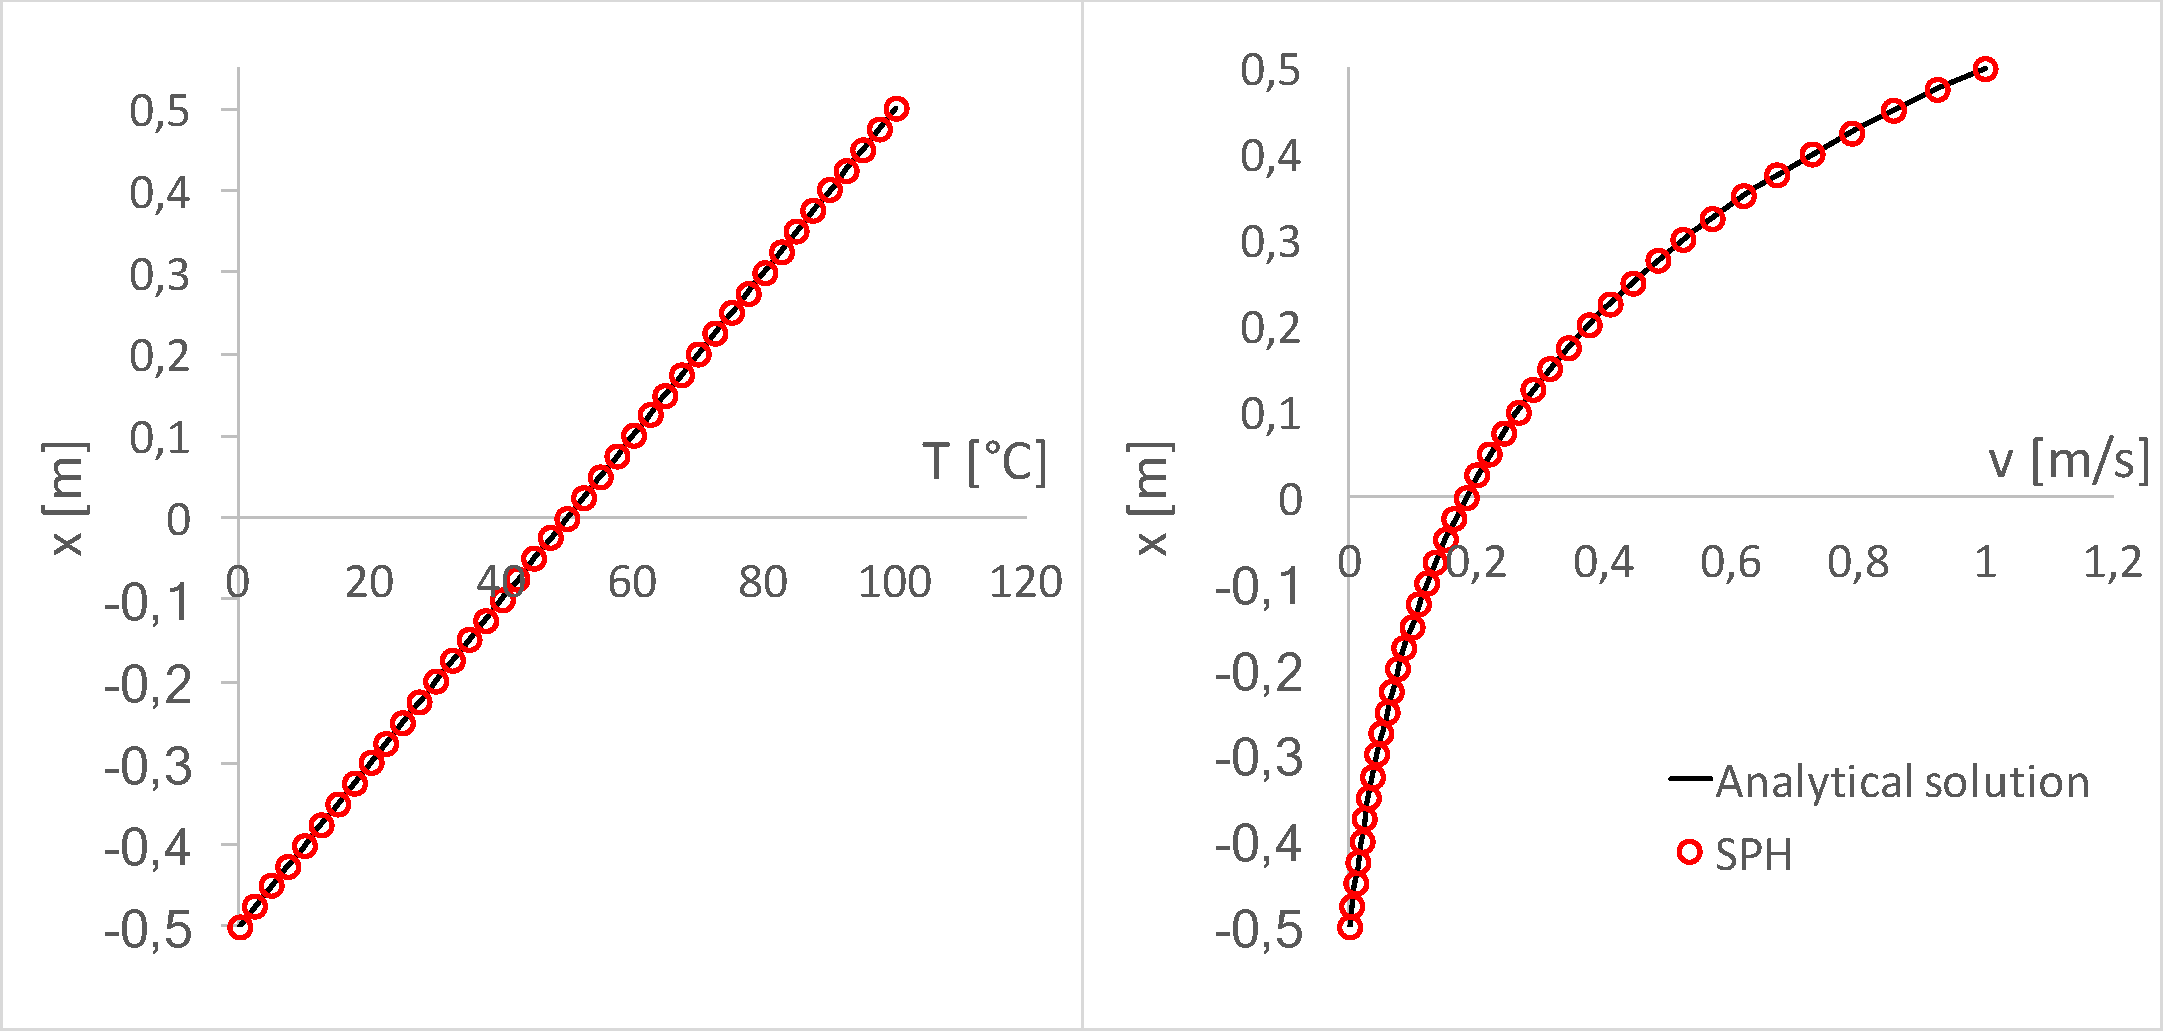
\includegraphics[scale=0.4]{couette_result.pdf}
  \centering
  \caption{Couette-flow results comparison.}
  \label{fig:couette_results}
\end{figure}\vspace*{3pt}

The results show very good agreement with the analytical solution in case of both the linear temperature and the exponential velocity distributions.
\subsection{Phase separation on a sphere}
\subsubsection{Problem definition}
The process of separation of two phases is usually modelled by the fourth order nonlinear Cahn-Hilliard equation
\begin{flalign} \label{eq:cahnhilliard}
\begin{split}
&\frac{\partial c}{\partial t}=D\Delta \mu,\\
&\mu=c^3-c-\gamma\Delta c, \\
\end{split}
\end{flalign}
where $c\in[-1,1]$ is the phase concentration, $\mu$ is the chemical potential, $\sqrt{\gamma}$ is the thickness of the transition region between the two phases and $D$ is a diffusion coefficient. In this particluar case the solution of equation \equref{eq:cahnhilliard} is investigated over a surface of a sphere.

\subsubsection{Numerical model and results}
The numerical scheme to discretise the system \equref{eq:cahnhilliard} is chosen to be SPH. Since the geometry is generated in Cartesian coordinates, the domain itself is three dimensional. However, the mollifier in the spatial interpolant should be two dimensional due to the interpretation of the problem on the spherical surface. The discretised form of the equations \equref{eq:cahnhilliard} are
\begin{flalign} \label{eq:cahnhilliard_sph_discretised}
\begin{split}
&\frac{\partial c_i}{\partial t}=D\sum_j{2(\mu_j-\mu_i)\frac{m_j}{\rho_j}\nabla W_{ij}},\\
&\mu_i=c^3-c-\gamma\sum_j{2(c_j-c_i)\frac{m_j}{\rho_j}\nabla W_{ij}}, \\
\end{split}
\end{flalign}
where again, $W_{ij}$ is normalised in two dimensions. The configuration file to solve \equref{eq:cahnhilliard_sph_discretised} is
\begin{example}{Cahn-Hilliard configuration file}{}
\lstset{basicstyle=\tiny}
\begin{lstlisting}[language=XML]
<?xml version="1.0" encoding="UTF-8"?>
<simulation>
  <case>
    <workspace>
      <constants>
        <L value="2"/>
        <dx value="0.0675"/>
        <csize value="dx*2.1"/>
        <rho0 value="1000"/>
        <mass value="dx^2*rho0"/>
        <D value="0.003"/>
        <CFL value="0.1"/>
        <gamma value="(csize/3)^2"/>
        <dt_g value="gamma/csize^2"/>
      </constants>
      <variables>
        <dt value="0.003"/>
        <Time value="0"/>
        <print_interval value="dt"/>
      </variables>
      <fields>
        <c value="rand(-1,1)"/> <!-- Initial condition -->
        <c_dot value="0"/>
        <mu value="0"/>
      </fields>
      <particle_system>
        <domain>
          <cell_size value="csize"/>
          <minimum value="-L/csize|-L/csize|-L/csize"/>
          <maximum value="L/csize|L/csize|L/csize"/>
          <boundary value="0|0|0"/>
        </domain>
        <grid>
          <gid value="0"/>  <!-- Read particle positions from file -->
          <file value="points.xyz"/>
        </grid>
      </particle_system>
    </workspace>
      <equations>
        <time value="Time=Time+dt"/>
        <chemical_potential value="mu=c^3-c-gamma*sph_L00(c,mass,rho0,Wp32220,csize)"/>
        <Cahn_Hilliard value="c_dot=D*sph_L00(mu,mass,rho0,Wp32220,csize)"/>
        <integration value="c=euler(c,c_dot,dt)"/>
        <new_dt value="dt=CFL*min(1/fmax(c_dot),dt_g)"/> <!-- Adaptive time stepping -->
        <print value="print_interval=exp(Time/45)"/> <!-- Modify printing interval -->
      </equations>
  </case>
  <parameter_space>
    <simulated_time value="150"/>
    <print_interval value="0.001"/>
    <confirm_on_exit value="false"/>
    <output_format value="BINARY"/>
  </parameter_space>
</simulation>

\end{lstlisting}
\end{example}
The phase separation process has a decaying intensity in the function of time, therefore the printing interval is adaptively modified with an exponential law to minimise the amount of simulation result files and keep the temporal sampling appropriate at the same time. The evolution of phase separation is shown in Figure \ref{fig:cahnhilliard_result} by the triangulation of the surface.
\begin{figure}[h!]
  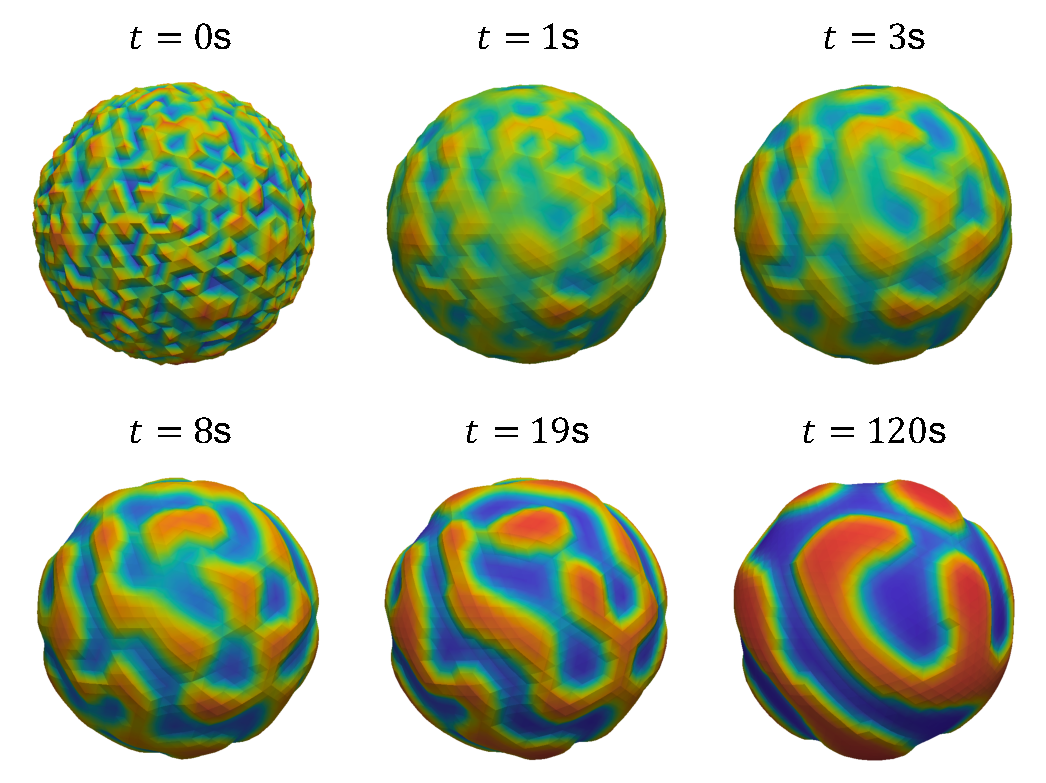
\includegraphics[scale=0.6]{cahnhilliard_result.pdf}
  \centering
  \caption{Evolution of phases on the sphere.}
  \label{fig:cahnhilliard_result}
\end{figure}\vspace*{3pt}


\subsection{Particle damper}
Particle dampers are one of the widely investigated damper systems today. Although there exists several analytical models to design and scale a particle damper, the complexity of the problem still requires experimental and numerical investigation. The geometry of the tank, the number and sizes of particles, the materials, the operating frequency are only some of the huge amount of possibilities concerning the development of particle dampers.
\subsubsection{Problem definition}
This test case simulates a simple three-dimensional oscillating cubic shell filled with spheres of identical radii. The cube is initially at rest in the position $z_0=-0.05$ m. The layout of the particle damper is presented in Figure \ref{fig:particle_damper_geom}, furthermore the values of the introduced quantities are summarised in Table \ref{tbl:particle_damper_values}. The system is supported by the ideal linear spring  merely damped by the 
\begin{figure}[h!]
  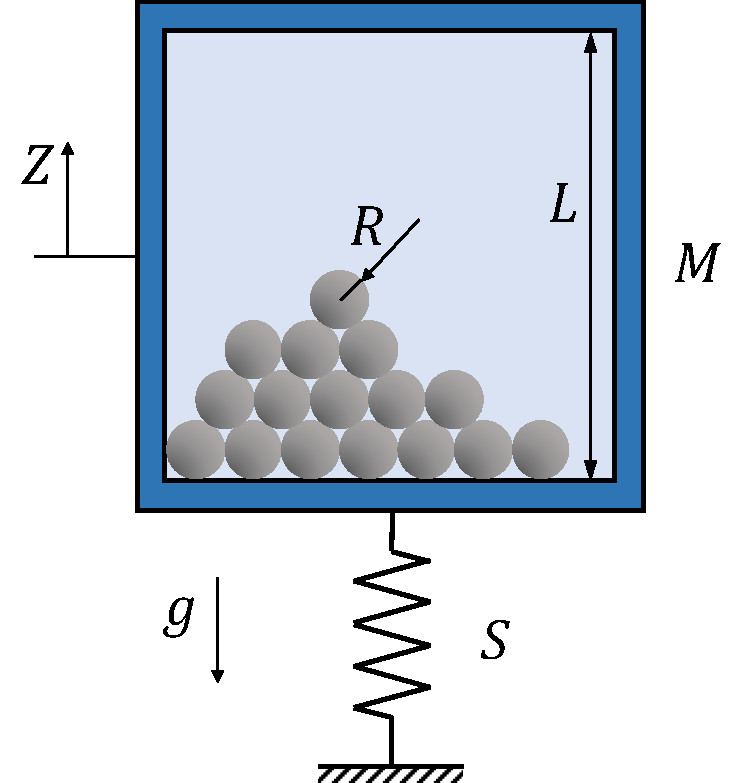
\includegraphics[scale=0.5]{particle_damper_geom.pdf}
  \centering
  \caption{Physical layout of the particle damper.}
  \label{fig:particle_damper_geom}
\end{figure}\vspace*{3pt}
\begin{table}[h!]
\begin{center}
\caption{Parameters of the particle damper simulation.}\label{tbl:particle_damper_values}
\begin{tabular}{ c l r } 
\toprule[1.5pt]
\bf Name & \bf Description & \bf Value \\
\midrule
$M$ & Cube mass & $20$ kg \\
$s$ & Spring stiffness & $78956.8$ kg/s$^2$ \\
$R$ & Particle radius & $4$ mm \\
$L$ & Cube edge length & $0.1$ m \\
$\rho$ & Particle mass density & $7850$ kg/m$^3$ \\
$E$ & Particle Young modulus & $2.06$ MPa \\
$\nu$ & Particle Poisson's ratio & $0.33$ \\
$g$ & Gravitational acceleration & $-9.81$ m/s${^2}$ \\
$N$ & Number of particles & 567 \\
\bottomrule[1.25pt]
\end{tabular}
\end{center}
\end{table}
\subsubsection{Numerical model and results}
A simple representaion of the physical model is introduced in this section with the notation that other valid solutions are also possible. To simplify the model and lacking the cube the simulation domain is chosen to be the interior of the cube. Since the domain is fixed, this assumption means that the simulation of the particle motion and collision is interpreted in the moving coordinate system associated to the cube and the excitation of the particles is governed purely by a time-dependent acceleration field superposed with the gravitational acceleration. The boundaries of the domain are set to symmetric, which plays an important role in the calculation of the forces acting on the cube. For the sake of simplicity the angular momentum of the particles is neglected.
The one-dimensional equation of motion of the cube is
\begin{flalign} \label{eq:cube_ode}
\begin{split}
M\ddot{Z}+SZ=F(t), \\
F(t) = -\sum_i{f_i}
\end{split}
\end{flalign}
where $F(t)$ is the resultant of the particle forces $f_i$. The solution of the homogeneous part of \equref{cube_ode} is the harmonic function
\begin{flalign} \label{eq:cube_sol}
Z(t)=C_1sin(\gamma t)+C_2cos(\gamma t),
\end{flalign}
where $C_1$ and $C_2$ are constants depending on the initial conditions and $gamma=\sqrt(S/M)$. Due to the lack of damping, the oscillation has constant amplitude. The particles' motion is determined by
\begin{flalign} \label{eq:spheres_ode}
\ddot r_i=\frac{1}{m_i}\sum_j{F^c(r_{ji},v_{ji},...)}+\frac{1}{m_i}\sum_j{F^b(r_{ji},v_{ji},...)}+g=\frac{1}{m_i}\sum_j{F^c(r_{ji},v_{ji},...)}+\frac{f_i}{m_i}+g,
\end{flalign}
where $F^c$ denotes the collection of the introduced collision laws introduced in Section \ref{sec:DEM_intro}. The second term on the RHS of \equref{eq:spheres_ode} operates with the same collision laws at the symmetric boundaries, which in turn contributes to \equref{eq:cube_ode}.
During the simulation the cube position, velocity and acceleration has to be calculated at each time steps. These quantities are considered as variables and calculated by the numerical solution of \equref{cube_ode}. The configuration file for the particle damper problem is as follows:
\begin{example}{Particle damper configuration file}{}
\lstset{basicstyle=\tiny}
\begin{lstlisting}[language=XML]
<?xml version="1.0" encoding="UTF-8"?>
<simulation>
  <case>
    <workspace>
      <constants>
        <L value="0.1"/>
        <csize value="0.01"/>
        <R value="0.004"/>
        <mass value="7850*4/3*R^3*pi"/>
        <E value="2.06e6"/>
        <nu value="0.33"/>
        <M value="20"/>
        <freq value="10"/>
        <gamma value="10*2*pi"/>
        <S value="gamma^2*M"/>
        <g value="0|0|-9.81"/>
      </constants>
      <variables>
        <T value="0"/>
        <dt value="5e-4"/>
        <A value="0"/>
        <V value="0"/>
        <Z value="-0.05"/>
      </variables>
      <particle_system>
        <domain>
          <cell_size value="csize"/>
          <minimum value="-L/2/csize|-L/2/csize|-L/2/csize"/>
          <maximum value="L/2/csize|L/2/csize|L/2/csize"/>
          <boundary value="symmetric|symmetric|symmetric"/>
        </domain>
        <grid>
          <gid value="0"/>
          <gpos value="-9*R|-9*R|-L/2"/>
          <gsize value="18*R|18*R|14*R"/>
          <goffset value="R|R|R"/>
          <gip_dist value="2*R|2*R|2*R"/>
        </grid>
      </particle_system>
      <fields>
        <a value="0|0|0"/>
        <v value="rand(-0.2,0.2)|rand(-0.2,0.2)|rand(-0.2,0.2)"/>
        <om value="0|0|0"/>
        <vproba value="V"/>
        <rproba value="Z"/>
      </fields>
    </workspace>
      <equations>
        <time value="T=T+dt"/>
        <eq value="a=dem_l(v,om,R,mass,E,nu,0,0.1)/mass"/>
        <tank_acceleration value="A=(-transpose(fsum(a)*mass)*e_k-S*Z)/M"/>
        <iv value="v=euler(v,a+g-A*e_k,dt)"/>
        <ia value="r=euler(r,v,dt)"/>
        <tank_velocity value="V=euler(V,A,dt)"/>
        <tank_position value="Z=euler(Z,V,dt)"/>
        <afsdf value="vproba=V"/>
        <afkms value="rproba=Z"/>
      </equations>
  </case>
  <parameter_space>
    <simulated_time value="1"/>
    <print_interval value="10*dt"/>
    <confirm_on_exit value="0"/>
    <output_format value="ASCII"/>
  </parameter_space>
</simulation>
\end{lstlisting}
\end{example}
After running the configuration file in Nauticle the individual particle elevation are visualised in Figure \ref{fig:particle_damper_result} together with the bottom and top positions of the tank.
\begin{figure}[h!]
  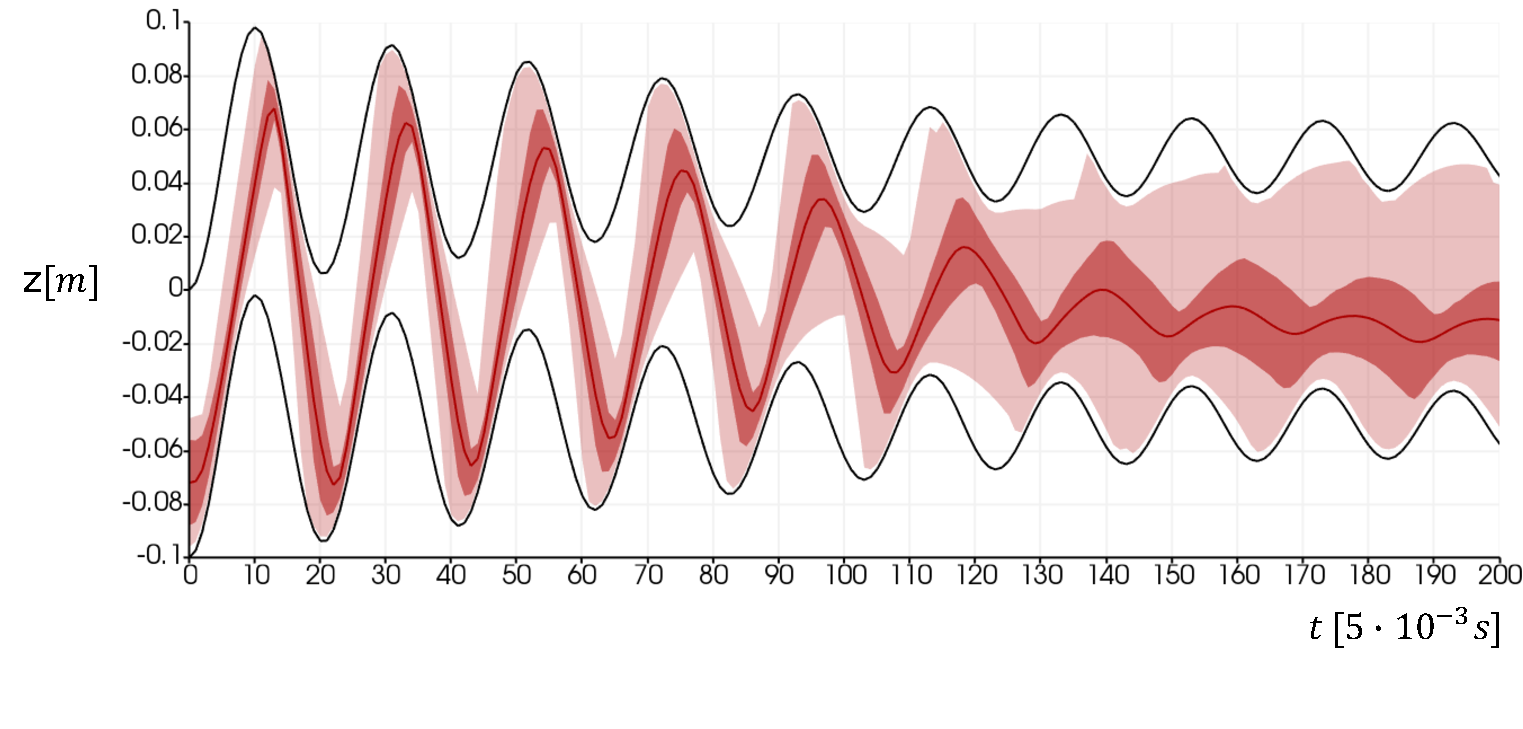
\includegraphics[scale=0.6]{particle_damper_time_series.pdf}
  \centering
  \caption{Particle (red) and tank (black) elevation in the function of time.}
  \label{fig:particle_damper_geom}
\end{figure}\vspace*{3pt}
As it is seen the oscillation amplitude is being reduced significantly until the particles start to gather at the bottom due to the smaller oscillation.


\subsection{Shear layer instability}
\subsection{Solar System}
The simulation of the solar System is a typical case of the n-body problem. The size of the objects are negligible and all objects are in interaction with all the others, consequently, the equation of motion \equref{nbody_eom} stands for all objects.
Due to the space-time scale of the Solar System it is recommended to deviate from SI units to decrease the inaccuracy of floating point arithmetics. Here the unit mass is equal to the mass of Earth (am), the unit distance is considered as the average distance of the Sun and the Earth (al) and finally, the unit length of time is one Earth-day (at). These units are summarised in Table \ref{tbl:astronomical_units}.
\begin{table}
\begin{center}
\caption{Units in the Solar System simulation.}\label{tbl:astronomical_units}
\begin{tabular}{ l r r }
\toprule[1.5pt]
\bf Name & \bf Unit & \bf Value \\
\midrule
Mass & am & $1.48093\cdot 10^{11}$kg \\
Length & al & $5.97\cdot 10^{24}$m \\
Time & at & $86400$s \\
\bottomrule[1.25pt]
\end{tabular}
\end{center}
\end{table}
Hence the gravitational constant is obtained as $\gamma=9.16324149\cdot 10^{-10}\rm{al}^3/(\rm{am}\cdot \rm{at}^2)$. The initial conditions of the Solar System is set to its state at 26 February 2000 00:00 (in heliocentric coordinates) introduced in Table \ref{tbl:solarsystempos} and \ref{tbl:solarsystemvel}. 
\begin{table}
\begin{center}
\caption{Mass of the Solar System planets.}\label{tbl:solarsystemmass}
\begin{tabular}{ l r }
\toprule[1.5pt]
\bf Object & \bf Mass [am] \\
\midrule
Sun & $3.32965046E+05$ \\
Mercury & $5.52604794E-02$ \\
Venus & $8.14805143E-01$ \\
Earth & $1.00000000E+00$ \\
Mars & $1.07447770E-01$ \\
Jupiter & $3.17831793E+02$ \\
Saturn & $9.51620463E+01$ \\
Uranus & $1.45359582E+01$ \\
Neptune & $1.71471140E+01$ \\
Pluto & $2.19381947E-03$ \\
\bottomrule[1.25pt]
\end{tabular}
\end{center}
\end{table}

\begin{table}
\begin{center}
\caption{Positions of the Solar system planets.}\label{tbl:solarsystempos}
\begin{tabular}{ l r r r }
\toprule[1.5pt]
\bf Object & \multicolumn{3}{c}{\bf Position [al]} \\
\midrule
Sun & $0.00000000E+00$  &  $0.00000000E+00$  &  $0.00000000E+00$ \\
Mercury & $-2.52875447E-01$  &  $1.89224913E-01$  &  $1.27303389E-01$ \\
Venus & $1.76553728E-02$  &  $-6.69151143E-01$  &  $-3.02159352E-01$ \\
Earth & $-9.18428887E-01$  &  $3.62942965E-01$  &  $1.57355594E-01$ \\
Mars & $1.21524135E+00$  &  $7.34458249E-01$  &  $3.04013819E-01$ \\
Jupiter & $3.77100459E+00$  &  $3.08343707E+00$  &  $1.22979557E+00$ \\
Saturn & $6.22706292E+00$  &  $6.43146103E+00$  &  $2.38855445E+00$ \\
Uranus & $1.47277740E+01$  &  $-1.24945774E+01$  &  $-5.68075252E+00$ \\
Neptune & $1.71271712E+01$  &  $-2.31196703E+01$  &  $-9.88938537E+00$ \\
Pluto & $-9.80572133E+00$  &  $-2.83258746E+01$  &  $-5.88297808E+00$ \\
\bottomrule[1.25pt]
\end{tabular}
\end{center}
\end{table}

\begin{table}
\begin{center}
\caption{Velocities of the Solar system planets.}\label{tbl:solarsystemvel}
\begin{tabular}{ l r r r }
\toprule[1.5pt]
\bf Object & \multicolumn{3}{c}{\bf Velocity [al/at]} \\
\midrule
Sun & $0.00000000E+00$  &  $0.00000000E+00$  &  $0.00000000E+00$ \\
Mercury & $-2.46358641E-02$  &  $-1.86902265E-02$  &  $-7.42852534E-03$ \\
Venus & $2.02895362E-02$  &  $8.45044680E-04$  &  $-9.03879795E-04$ \\
Earth & $-7.15783449E-03$  &  $-1.47042339E-02$  &  $-6.37503091E-03$ \\
Mars & $-7.19683749E-03$  &  $1.17815694E-02$  &  $5.59840572E-03$ \\
Jupiter & $-5.13821923E-03$  &  $5.54945851E-03$  &  $2.50386823E-03$ \\
Saturn & $-4.47179956E-03$  &  $3.42854338E-03$  &  $1.60843860E-03$ \\
Uranus & $2.67440395E-03$  &  $2.51272963E-03$  &  $1.06268844E-03$ \\
Neptune & $2.59474895E-03$  &  $1.69891959E-03$  &  $6.30906866E-04$ \\
Pluto & $3.06493917E-03$  &  $-1.12260841E-03$  &  $-1.27466162E-03$ \\
\bottomrule[1.25pt]
\end{tabular}
\end{center}
\end{table}

\subsection{Lid-driven cavity}
\subsubsection{Problem definition}
One of the most famous test cases of SPH is the two dimensional wall-driven flow inside a square cavity with edge length $L$. The geometry of the cavity and is presented in Figure \ref{fig:liddrivencavitysph}. 
\begin{figure}[h!]
  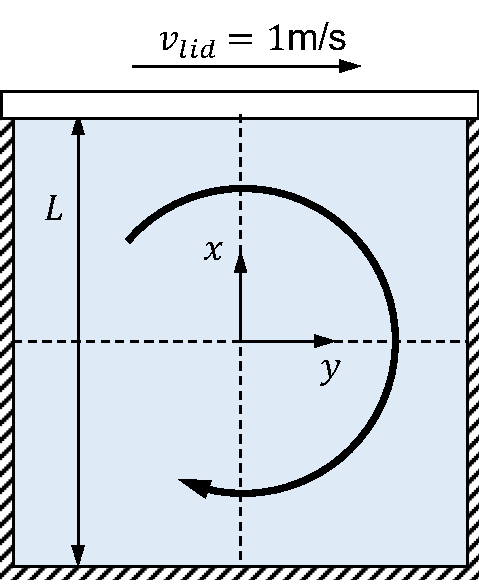
\includegraphics[scale=0.6]{liddrivencavity.pdf}
  \centering
  \caption{2D flow in a square cavity driven by the lid.}
  \label{fig:liddrivencavitysph}
\end{figure}\vspace*{3pt}

In Lagrangian frame the governing equations of the fluid can be written as
\begin{flalign} \label{eq:liddrivencavitysph}
\begin{split}
&\nabla v=0, \\
&\frac{dv}{dt}=\frac{1}{\rho}\nabla p+\nu\Delta v, \\
\end{split}
\end{flalign}
where $p$ and $\rho$ are the pressure and density of the fluid, $v$ is the Lagrangian fluid velocity and $\nu$ is the physical kinematic viscosity of the fluid. The corresponding no-slip boundary conditions demand the velocity constraints
\begin{flalign} \label{eq:liddrivencavitysphbc}
\begin{split}
&v\bigg(\pm\frac{L}{2},y\bigg)=0, \\
&v\bigg(x,-\frac{L}{2}\bigg)=0, \\
&v_y\bigg(x,\pm\frac{L}{2}\bigg)=0, \\
&v_x\bigg(x,\frac{L}{2}\bigg)=v_{lid}, \\
\end{split}
\end{flalign}
where $v_{lid}$ is the velocity of the closing lid over the cavity.
\subsubsection{Numerical model and results}
The discretised form of the equations \equref{eq:liddrivencavitysph} can be constructed similarly to the former SPH test cases:
\begin{flalign} \label{eq:dambreak_sph_discretised}
\begin{split}
&\frac{d\rho_i}{dt}=-\rho_i\sum{(v_j-v_i)\frac{m_j}{\rho_j}\nabla W_{ij}}+0.1hc\sum_j{2(\rho_j-\rho_i)\frac{r_{ij}}{|r_{ij}|^2}\frac{m_j}{\rho_j}\nabla W_{ij}}, \\
&\frac{dv_i}{dt}=-\sum_j{\bigg(\frac{p_i}{\rho_i^2}+\frac{p_j}{\rho_j^2}\bigg)m_j\nabla W_{ij}}+\nu\sum_j{2(v_j-v_i)\frac{r_{ij}}{|r_{ij}|^2}\frac{m_j}{\rho_j}\nabla W_{ij}}, \\
\end{split}
\end{flalign}
where $h$ is the smoothing distance of the kernel function $W_{ij}$. The second term on the RHS of the equations \equref{eq:dambreak_sph_discretised} is the artificial density and velocity diffusion term respectively. The application of the density diffusion term is often referred as the $\delta$-SPH formulation. Since the equations \equref{eq:dambreak_sph_discretised} do not imply constraint between the velocity and pressure fields, an additional state equation
\begin{equation} \label{eq:eos}
p_i=c^2(\rho-\rho_0)+p_0,
\end{equation}
is required to couple the equations, where $\rho_0$ is the rest density of the fluid, $p_0$ is the background pressure and $c$ is the speed of acoustic waves artificially reduced to ensure numerical stability. Although exact incompressibility cannot be achieved using \equref{eq:eos}, the density variation can be limited to $\delta\rho=1\%$ by choosing $c=10v_{lid}$.




\subsection{Granular material}
\subsection{Biharmonic equation}


\section{The Nauticle open-source code}
This section comments the role of each source and header file of Nauticle. For better clarity the explanation is divided into different groups marked by the subsequent sections.
\subsection{Nodes of the expression tree}
\subsubsection{Particlewise nodes}
\textbf{pmExpression.h / pmExpression.cpp} \\
Declares / defines the expression node of the expression tree. This is an abstract class. \\

\textbf{pmSymbol.h / pmSymbol.cpp} \\
Declares / defines the symbol node of the expression tree. This is an abstract class. \\

\textbf{pmSingle.h / pmSingle.cpp} \\
Declares / defines the single node of the expression tree. This is an abstract class. \\

\textbf{pmConstant.h / pmConstant.cpp} \\
Declares / defines the node for constants in the expression tree. \\

\textbf{pmVariable.h / pmVariable.cpp} \\
Declares / defines the node for variables in the expression tree. \\

\textbf{pmField.h / pmField.cpp} \\
Declares / defines the field node of the expression tree. \\

\textbf{pmParticle\_system.h / pmParticle\_system.cpp} \\
Declares / defines the particle system node of the expression tree. It performs neighbour searching. \\

\textbf{pmArithmetic\_function.h} \\
Declares / defines the node for arithmetic functions in the expression tree. \\

\textbf{pmArithmetic\_operator.h} \\
Declares / defines the node for arithmetic operators in the expression tree. \\


\subsubsection{Nodes for interaction branch}
\textbf{pmInteraction.h} \\
Declares / defines the interaction node in the expression tree. This is an abstract class. It manages the interparticle connections. \\

\textbf{pmFsearch.h / pmFsearch.cpp} \\
Declares / defines the class for field search algorithms. This is an abstract class. \\

\textbf{pmFmin.h / pmFmin.cpp} \\
Declares / defines the functions for minimum search of a field.  \\

\textbf{pmFmax.h / pmFmax.cpp} \\
Declares / defines the functions for maximum search of a field. \\

\textbf{pmFmean.h / pmFmean.cpp} \\
Declares / defines the functions for mean calculation of a field. \\

\textbf{pmFsum.h / pmFsum.cpp} \\
Declares / defines the functions for sum calculation of a field. \\

\textbf{pmNbody.h / pmNbody.cpp} \\
Declares / defines the functions for particle interactions. It calculates the gravitational forces. \\

\textbf{pmNeighbours.h / pmNeighbours.cpp} \\
Declares / defines the functions for particle interactions. It calculates the number of neighbours in a given distance. \\

\textbf{pmDem.h} \\
Declares / defines the node in the expression tree to calculate interactions based on Discrete Element Method (DEM). \\

\textbf{pmOperator.h} \\
Declares / defines the operator node in the expression tree. This is an abstract class. \\

\textbf{pmFilter.h} \\
Declares / defines the Filter node in the expression tree. This is an abstract class. \\

\textbf{pmSph\_operator.h} \\
Declares / defines functions for SPH interactions and differential operators. \\

\subsubsection{Files for simulation case}

\textbf{pmCommand\_parser.h / pmCommand\_parser.cpp} \\
Declares / defines the functions that manage terminal commands. \\

\textbf{pmTensor.h / pmTensor.cpp} \\
Declares / defines the class that implements functions for tensor quantities. \\

\textbf{pmTensor\_parser.h / pmTensor\_parser.cpp} \\
Declares / defines the functions that analyse tensors based on expressions. \\

\textbf{pmParameter\_space.h / pmParameter\_space.cpp} \\
Declares / defines the functions for parameter management. \\

\textbf{pmCase\_manager.h / pmCase\_manager.cpp} \\
Declares / defines the functions that read the configuration file, build and run the simulation through the solver. \\

\textbf{pmDomain.h / pmDomain.cpp} \\
Declares / defines the rectangular simulation domain class in which the particles exist. \\

\textbf{pmMath\_parser.h / pmMath\_parser.cpp} \\
Declares / defines the functions for string parsing. \\

\textbf{pmMath\_test.h / pmMath\_test.cpp} \\
Declares / defines the class that performs mathematical expressions stored in string format. This is an abstract class. \\

\textbf{pmExpression\_parser.h / pmExpression\_parser.cpp} \\
Declares / defines the functions for expression parsing. \\

\textbf{pmEquation\_parser.h / pmEquation\_parser.cpp} \\
Declares / defines the class that analyses user defined equations of the configuration file. \\

\textbf{pmEquation.h / pmEquation.cpp} \\
Declares / defines the class for user defined equations. It contains two expressions (LHS and RHS). It performs the evaluation too. \\

\textbf{pmWorkspace.h / pmWorkspace.cpp} \\
Declares / defines the class that manages user defined variables, constants, fields, and particle system. \\

\textbf{pmCase.h / pmCase.cpp} \\
Declares / defines the class that manages the workspace and user defined equations (UDE's). It also solves the equations. \\

\textbf{pmGrid.h / pmGrid.cpp} \\
Declares / defines the class for particle generation. Two ways: rectangular grid or particles from .xyz file. \\

\textbf{pmGrid\_space.h / pmGrid\_space.cpp} \\
Declares / defines the class that manages, merges grids. \\

\textbf{pmVTK\_manager.h / pmVTK\_manager.cpp} \\
Declares / defines the functions for VTK reading and writing. This is an abstract class. \\

\textbf{pmVTK\_reader.h / pmVTK\_reader.cpp} \\
Declares / defines the functions for VTK reading. \\

\textbf{pmVTK\_writer.h / pmVTK\_writer.cpp} \\
Declares / defines the functions for VTK writing. \\

\textbf{pmXML\_processor.h / pmXML\_processor.cpp} \\
Declares / defines the functions for extracting data from xml file. \\

\subsubsection{Other files}
\textbf{pmRandom.h / pmRandom.cpp} \\
Declares / defines the functions for random number generation in a range. \\

\textbf{pmLog\_stream.h / pmLog\_stream.cpp} \\
Declares / defines the class that manages logging into file and terminal. \\

\textbf{pmSort.h}\\
Implements functions for sorting and reordering.\\

\textbf{pmKernel.h / pmKernel.cpp} \\
Declares / defines the functions for SPH kernels.\\

\textbf{pm.h}\\
Wraps includes.\\

\textbf{pmNoncopyable.h}\\
Implements a class for objects that are not allowed to be copied.\\

\textbf{pmVersion.h}\\
Contains Nauticle major and minor version information.\\


\section{Licenses}
\subsection{VTK license}
VTK is an open-source toolkit licensed under the BSD license.\\
Copyright (c) 1993-2008 Ken Martin, Will Schroeder, Bill Lorensen \\
All rights reserved.\\
Redistribution and use in source and binary forms, with or without modification, are permitted provided that the following conditions are met: \\
- Redistributions of source code must retain the above copyright notice, this list of conditions and the following disclaimer. \\
- Redistributions in binary form must reproduce the above copyright notice, this list of conditions and the following disclaimer in the documentation and/or other materials provided with the distribution. \\
- Neither name of Ken Martin, Will Schroeder, or Bill Lorensen nor the names of any contributors may be used to endorse or promote products derived from this software without specific prior written permission.\\

THIS SOFTWARE IS PROVIDED BY THE COPYRIGHT HOLDERS AND CONTRIBUTORS “AS IS” AND ANY EXPRESS OR IMPLIED WARRANTIES, INCLUDING, BUT NOT LIMITED TO, THE IMPLIED WARRANTIES OF MERCHANTABILITY AND FITNESS FOR A PARTICULAR PURPOSE ARE DISCLAIMED. IN NO EVENT SHALL THE AUTHORS OR CONTRIBUTORS BE LIABLE FOR ANY DIRECT, INDIRECT, INCIDENTAL, SPECIAL, EXEMPLARY, OR CONSEQUENTIAL DAMAGES (INCLUDING, BUT NOT LIMITED TO, PROCUREMENT OF SUBSTITUTE GOODS OR SERVICES; LOSS OF USE, DATA, OR PROFITS; OR BUSINESS INTERRUPTION) HOWEVER CAUSED AND ON ANY THEORY OF LIABILITY, WHETHER IN CONTRACT, STRICT LIABILITY, OR TORT (INCLUDING NEGLIGENCE OR OTHERWISE) ARISING IN ANY WAY OUT OF THE USE OF THIS SOFTWARE, EVEN IF ADVISED OF THE POSSIBILITY OF SUCH DAMAGE.

\subsection{Nauticle}
\noindent
Copyright \textcopyright{} 2016-2017 by Balazs Toth \\
\noindent
BME Budapest University of Technology and Economics, Department of Hydraulic and Water Resources Engineering\\

Nauticle is free software: you can redistribute it and/or modify it under the terms of the GNU Lesser General Public License as published by the Free Software Foundation, either version 3 of the License, or (at your option) any later version Nauticle is distributed in the hope that it will be useful, but WITHOUT ANY WARRANTY; without even the implied warranty of MERCHANTABILITY or FITNESS FOR A PARTICULAR PURPOSE.  See the GNU Lesser General Public License for more details You should have received a copy of the GNU Lesser General Public License along with Nauticle.  If not, see \myhref{http://www.gnu.org/licenses/}{http://www.gnu.org/licenses/}\\
 For more information please visit: \myhref{https://bitbucket.org/Nauticleproject/}{https://bitbucket.org/Nauticleproject/}


\end{document}